\documentclass [11pt]{article}
\usepackage {amssymb}
\usepackage {amsmath}
\usepackage {graphicx}

\setlength{\textwidth}{6.25in}
\setlength{\textheight}{8.75in}
\setlength{\evensidemargin}{0in}
\setlength{\oddsidemargin}{0in}
\setlength{\topmargin}{0.2in}
\setlength{\parskip}{.1in}  
\setlength{\parindent}{0.0in}  


%\renewcommand{\textfraction}{0.01}
%\renewcommand{\topfraction}{0.99}
%\renewcommand{\bottomfraction}{0.99}
%\renewcommand{\floatpagefraction}{0.99}


\pagestyle{headings}

\def\X{\mathbf{X}}
\def\A{\mathbf{A}}
\def\B{\mathbf{B}}
\def\C{\mathbf{C}}
\def\D{\mathbf{D}}
\def\S{\mathbf{S}}
\def\E{\mathbf{E}}
\def\I{\mathbf{I}}
\def\N{\mathbf{N}}


\def\x{\mathbf{x}}
\def\b{\mathbf{b}}
\def\u{\mathbf{u}}
\def\v{\mathbf{v}}
\def\w{\mathbf{w}}
\def\n{\mathbf{n}}
\def\p{\mathbf{p}}

\newcommand{\bv}{\vspace{-0.05in} \begin{verbatim}}
\newcommand{\ev}{\end{verbatim}}
\newcommand{\ttt}[1]{\texttt{#1}}
\newcommand{\tab}{\hspace*{0.5in}}
\newcommand{\lift}{\vspace{-0.15in}} 

\newcounter{exercise}
\numberwithin{exercise}{section}
\newcommand{\exnumber}{\addtocounter{exercise}{1} \theexercise \thinspace}

\begin{document}

\begin{center} 
\Large An introduction to \textbf{Matlab} for dynamic modeling \\
\normalsize Last compile: \today \\
\vspace{0.25in}
\large  
Stephen P. Ellner$^1$ and John Guckenheimer$^2$\\ 
${}^1$Department of Ecology and Evolutionary Biology, and \\
${}^2$Department of Mathematics \\
Cornell University \\
\normalsize \end{center}

\tableofcontents
\section*{Introduction} 
These notes for computer labs accompany our textbook \textit{Dynamic Models in Biology} (Princeton University
Press 2006). They are based in part on course materials 
by former TAs Colleen Webb, Jonathan Rowell and Daniel Fink at Cornell, 
Professors Lou Gross (University of Tennessee) and Paul Fackler (NC State University), and 
on the book \textit{Getting Started with Matlab} by Rudra Pratap (Oxford University Press). 
So far as we know, the exercises here and in the textbook can all be done using 
the Student Edition of Matlab, or a regular base license without additional
Toolboxes. 

Sections 1-7 are a general introduction to the basics of the Matlab language,
which we generally cover in 2 or 3 lab sessions, depending on how much previous
Matlab experience students have had. 
These contain many sample calculations. It is important to 
do these yourselves -- \textbf{type them in at your keyboard and see what
happens on your screen} -- to get the feel of working in Matlab. 
Exercises in the middle of a section should be done \textit{immediately} when you 
get to them, and make sure that you have them right 
before moving on. Exercises at the ends of these sections are often more
challenging and more appropriate as homework exercises. 

The subsequent sections are linked to our textbook, in fairly obvious ways. For example,
section \ref{MatComp} on matrix computations goes with Chapter 2 on matrix models for
structured populations, and section \ref{MLplane} on phase-plane analysis of the
Morris-Lecar model accompanies the corresponding section in Chapter 5 of the
textbook. The exercises here include some that are intended to be 'warmups' for
exercises in the book (e.g., simple examples of simulating discrete-event
models, as a warmup for doing discrete-event simulations of infectious disease
dynamics). 


The home for these notes is currently \texttt{www.cam.cornell.edu/$\sim$dmb/DMBsupplements.html},
a web page for the book that we maintain ourselves. If that fails, an up-to-date link should 
be in the book's listing at the publisher (\texttt{www.pupress.princeton.edu}).   
Parallel notes and script files using the open-source \textbf{R} language are being written -- email 
spe2@cornell.edu us if you would like to get these in their present imperfect state. Eventually 
(and certainly before the end of 2006) they will be posted alongside these. 

\section{Interactive calculations}
\vspace{-0.15in} 
The MATLAB interface is a set of interacting windows. In some of these you 
``talk" to MATLAB, and in others MATLAB ``talks" to you. Windows can be closed 
(the \textbf{$\times $} button) or detached to become free-floating (curved 
arrow button). To restore the original layout, use \textbf{View/Desktop 
Layout/Default} in the main menu bar. 

Two important windows are \textbf{Launch Pad} and \textbf{Command}. 
Launch Pad is the online Help system. The Command window is for  
\textit{interactive commands}, meaning that the command is executed and 
the result is displayed as soon as you hit the Enter key. For example, at 
the command prompt \ttt{>>}, type in 2+2 and hit Enter; you will see 
\begin{verbatim}
>> 2+2
ans =
     4
\end{verbatim}
Now type in 2+2; (including the semicolon) -- what happens? A semicolon at 
the end of a line tells MATLAB \textbf{not} to display the results of the 
calculation. This lets you do a long calculation (e.g. solve a model with 
a large number of intermediate results) and then display only the final result. 

To do anything complicated, the results have to be stored 
in variables. For example, type \texttt{a=2+2} in the Command window and you 
see 
\begin{verbatim}
>>  a=2+2
a =
    4
\end{verbatim}
The variable \texttt{a} has been created, and assigned the value 4. By 
default, a variable in MATLAB is a matrix (a rectangular array of numbers); 
in this case \texttt{a} is a matrix of size 1$\times $1 (one row, one 
column), which acts just like a number. 

Variable names must begin with a letter, and followed by up to 30 letters, 
numbers, or underscore characters. \textbf{Matlab is case sensitive}: 
\texttt{Abc} and \texttt{abc} are not the same variable. In contrast to
some other languages, a period (.) \textit{cannot} be part of a variable
name. 

\textbf{Exercise\exnumber} Here are some variable names that cannot
be used in Matlab; explain why: \texttt{cell.maximum.size; 4min; site\#7 .} 

Calculations are done with variables as if they were numbers. MATLAB uses 
\verb! +, -, *, /, and ^! for addition, subtraction, multiplication, division and 
exponentiation, respectively. For example enter
\begin{verbatim}
>>  x=5; y=2; z1=x*y, z2=x/y, z3=x^y
\end{verbatim} 
and you should see 
\begin{verbatim}
z1 =
    10
z2 =
    2.5000
z3 =
    25
\end{verbatim}
Notice that several commands can go on the same line. The first two were 
followed by semicolons, so the results were not displayed. The rest were 
followed by commas, and the results were displayed. A comma after the last 
statement on the line isn't necessary. 

Even though x and y were not displayed, MATLAB ``remembers" their values.  
Type \\
\tab \texttt{>> x, y}\\
and MATLAB displays the values of x and y. Variables defined in a session 
are displayed in the \textbf{Workspace} window. Click on the tab to activate 
it and then double-click on \texttt{x} to launch a window 
summarizing \texttt{x'}s properties and entries. Since \texttt{x} is a 
1$\times $1 matrix, there's only one value. Getting a bit ahead of 
ourselves, create a 3$\times $2 matrix of 1's with the command \\
\tab \texttt{>>  X=ones(3,2)}\\
and then look at what X is using the Workspace window. Clicking on the matrix
icon opens a window that displays its values.

Commands can be edited, instead of starting again from 
scratch. There are two ways to do this. In the Command window, the 
$\uparrow$ key recalls previous commands. For example, 
you can bring back the next-to-last command and edit it to 
\begin{verbatim}
>>  x=5 y=2 z1=x*y z2=x/y z3=x^y
\end{verbatim} 
so that commands are not separated by either a comma or semicolon. Then 
press Enter, and you will get an error message. \textit{Multiple commands on a 
line have to be separated by a comma or a semicolon (no display)}. 

The other way is to use the \textbf{Command History} 
window, which holds a running history of your commands. You can re-run a 
command by double-clicking on it. 

You can do several operations in one calculation, such as 
\begin{verbatim}
    >> A=3; C=(A+2*sqrt(A))/(A+5*sqrt(A))
    C =
        0.5544
\end{verbatim}
The parentheses are specifying the order of operations. The command 

\tab \texttt{>>  C=A+2*sqrt(A)/A+5*sqrt(A)} 

gets a different result -- the same as 

\tab \texttt{>>  C=A + 2*(sqrt(A)/A) + 5*sqrt(A)}. 

The default order of operations is: (1) Exponentiation, (2) multiplication 
and division, (3) addition and subtraction. Operations of equal priority are 
performed left to right.
\begin{verbatim}
>> b = 12-4/2^3          gives    12 - 4/8 = 12 - 0.5 = 11.5
>> b = (12-4)/2^3        gives    8/8 = 1
>> b = -1^2              gives    -(1^2) = -1
>> b = (-1)^2            gives    1 
\end{verbatim}
In complicated expressions it's best to use parentheses to specify 
explicitly what you want, such as \verb! >> b = 12 - (4/(2^3)) ! 
or at least \verb! >> b = 12 - 4/(2^3)!. \textbf{Use lots of parentheses} instead of
trusting the computer to figure out what you meant.  

MATLAB also has many \textbf{built-in mathematical functions} that operate on variables
(see Table \ref{MathFunctions}). You can get help on any function by entering \\
\hspace*{1in} \texttt{help functionname} \\
in the console window (e.g., try \texttt{help sin}). You should also explore
the items available on the Help menu. 
 
\begin{table}
\begin{tabular}{p{140pt}p{280pt}}
\hline
\hline
abs(x) & absolute value \\
cos(x), sin(x), tan(x) &  cosine, sine, tangent of angle x in radians\\
exp(x)  & exponential function  \\
log(x)  & natural (base-e) logarithm \\
log10(x) &  common (base-10) logarithm \\
sqrt(x)  &  square root \\
\hline
\hline  
\end{tabular}
\caption{Some of the built-in basic math functions in MATLAB. You can
get more complete lists from the Help menu or Launch Pad, organized by 
function name or by category.} 
\label{MathFunctions}
\end{table}

\textbf{Exercise\exnumber}: Have MATLAB compute the values of
\begin{enumerate} 
\item $\frac{2^5}{2^5 - 1}$and compare it with $\left( {1 - \frac{1}{2^5}} 
\right)^{ - 1}$ [answer: 1.0323] 
\item $\sin (\pi / 6), \cos^2(\pi / 8)$ [answers: 0.5, 0.8536. The constant $\pi$ is
a pre-defined variable \texttt{pi} in Matlab. So typing \texttt{cos(pi/8)} works in Matlab,
but note that \texttt{cos$\wedge$2(pi/8)} won't work!] 
\item $\frac{2^5}{2^5 - 1}+4\sin (\pi / 6)$ [answer: 3.0323]. 
\end{enumerate} 

\textbf{Exercise\exnumber} Use the Help system to find out what
the \textbf{hist} function does -- most easily, by typing \texttt{help hist}
at the command prompt. After you do that, type \texttt{doc hist} and see what
happens (if the formatted help pages are installed on your computer, you'll get one of them). 
Prove that you have succeeded by doing the following: use the command \ttt{y=randn(5000,1);} to generate
a vector of 5000 random numbers with a Normal distribution, and then
use \ttt{hist} to plot a histogram of the values in \ttt{y} with 21 bins. 

\section{An interactive session: linear regression}
\vspace{-0.15in} 
To get the feel of working in MATLAB, we'll fit a straight-line descriptive model to some data
(i.e., we will do a simple linear regression). The latest version of Matlab lets you do straight-line fitting 
by point-and-click, but you don't learn much about Matlab by doing it that way.     

Below are some data on the maximum growth rate \textit{rmax} 
of laboratory populations of the green alga \textit{Chlorella vulgaris} as a function of light 
intensity ($\mu$E per m$^2$ per second). 

\tab Light: 20,  20,  20,  20,  21,  24,  44,  60,  90,  94, 101 \\
\tab rmax: 1.73, 1.65, 2.02, 1.89, 2.61, 1.36, 2.37, 2.08, 2.69, 2.32, 3.67 

To analyze these data in MATLAB, first enter them into \textit{vectors}: 
\begin{verbatim}
>> Light=[20 20 20 20 21 24 44 60 90 94 101]
>> rmax=[1.73 1.65 2.02 1.89 2.61 1.36 2.37 2.08 2.69 2.32 3.67]
\end{verbatim}

A vector is a list of numbers. The commands above entered Light and rmax as \textit{row vectors}. 
Double-click on Light and rmax in the Workspace window and you'll see that they are 
stored in MATLAB as 1$\times $11 matrices, i.e. a matrix with a single row. 
To see a histogram of the light intensities \\
\tab \texttt{>> hist(Light)} \\
opens a graphics window and displays the histogram. There are some other 
built-in statistics functions, for example \texttt{\textbf{mean(Light)}}gets you 
the mean, \texttt{\textbf{std(Light)}} returns the standard deviation. 

Now to see how light intensity and rmax are related, 

\tab \texttt{>>  plot(Light,rmax,'+')}

creates a plot with the data points indicated by + symbols. A linear 
regression seems reasonable. The MATLAB function \textbf{polyfit} calculates the 
regression coefficients: \\
\tab \texttt{>>  C=polyfit(Light,rmax,1) } \\
gets you 
\begin{verbatim}
C =
    0.0136    1.5810
\end{verbatim}
\texttt{polyfit(Light,rmax,1)}means that we have fitted a first-degree polynomial 
(a line) with Light as the x-variable and rmax as the y-variable. The vector 
C is returned with 0.0136 being the slope and 1.5810 the y-intercept. 

Graphing the regression line takes a bit of work. First, we need to pick 
some values at which to calculate values of the regression line [really we 
only need two points to plot a line, so the following is to illustrate 
plotting curves in general]. Using \\
\tab \texttt{>>  min(Light), max(Light) } \\
we find that Light runs from 20 to 101, so we could use \\
\tab \texttt{>>  xvals=0:120;} 

This makes xvals a vector of the integers from 0 to 120. Then \\
\tab \texttt{>>  yhat=polyval(C,xvals);} \\
uses the coefficients in C to calculate the regression line at the values in 
xvals. Finally, to plot the data and regression curve on one graph: 

\tab \texttt{>> plot(Light,rmax,'+',xvals,yhat)}

That looks pretty good. If you feel like it, use the menus on the graph 
window to add axis labels like those in the figure below (use the 
\textbf{Insert} menu) and the regression equation (click on the \textbf{A 
}to create a text box). 

\begin{figure}[htbp]
\centerline{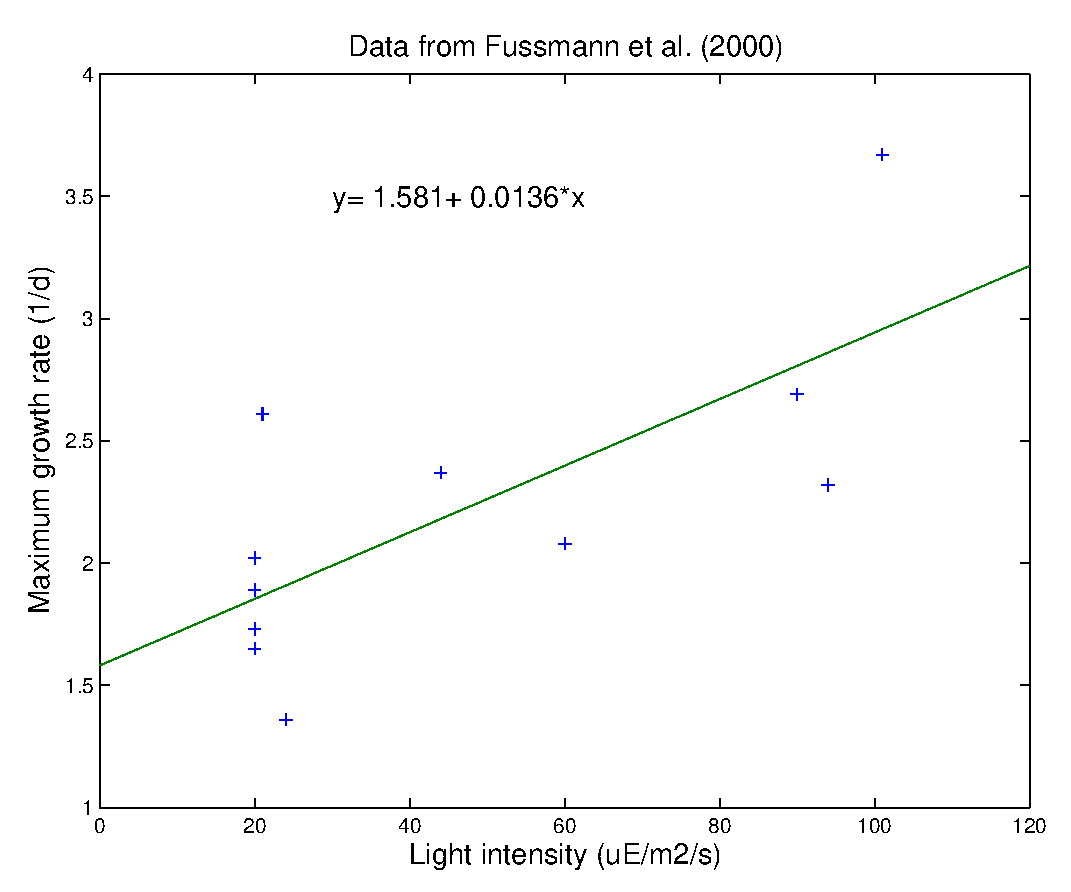
\includegraphics[width=4in]{figures/MatlabIntro1.eps}}
\caption{Graph produced by Intro1.m, with some labels and text added. Data are from the 
studies described in the paper: G. Fussmann, S.P. Ellner, K.W. Shertzer, and N.G. Hairston, Jr. 2000. 
Crossing the Hopf bifurcation in a live predator-prey system. Science 290: 1358-1360.} 
\label{fig1}
\end{figure}

\section{M-files and data files}
\vspace{-0.15in} 
Small tasks can be done interactively, but modeling or complicated data 
analysis are done using \textit{programs} -- sets of commands stored in a file. 
MATLAB uses the extension \textbf{.m} for program files and refers to them 
as \textbf{M-files}. 

Most programs for working with models or analyzing data follow a
simple pattern:
\begin{enumerate}
\item ``Setup'' statements.
\item Input some data from a file or the keyboard.
\item Carry out the calculations that you want.
\item Print the results, graph them, or save them to a file.
\end{enumerate}
As a first example, get a copy of \textbf{Intro1.m} which has the commands from the 
interactive regression analysis. One good place to put downloaded files is 
Matlab's \textbf{work} folder, which is the default location for user 
files.

Now use \textbf{File/Open} in Matlab to open your copy of 
\textbf{Intro1.m}, which will be loaded into the \textit{M-file editor window.} In that window, select 
\textbf{Run} on the \textbf{Debug} menu, and the commands in the file will 
be executed, resulting in a graph being displayed with the results. 

M-files let you build up a calculation step-by-step, making sure that each 
part works before adding on to it. For example, in the last line of 
\textbf{Intro1.m }change \texttt{yhat }to \texttt{ygat}:

\tab \texttt{>>  plot(Light,rmax,'+',xvals,ygat)}

Run the file again and look at the Command Window. The variable 
\texttt{ygat} doesn't exist, and MATLAB gives you an error message. Now 
change it back to \texttt{yhat} and re-run the file. 

Another important time-saver is loading data from a text file. Get copies   
of \textbf{Intro2.m} and \textbf{ChlorellaGrowth.txt} 
to see how this is done. First, instead of having to type in
the numbers at the Command line, the command

\tab \texttt{X=load('ChlorellaGrowth.txt')}

reads the numbers in \textbf{ChlorellaGrowth.txt} and puts them into variable 
\textbf{X}. We extract them with 
the commands

\tab \texttt{Light=X(:,1); rmax=X(:,2);}

These are shorthand for 'Light=everything in column 1 of X', and 
'rmax=everything in column 2 of X' (we'll learn more about working with 
matrices later). From there out it's the same as before, followed by a few lines that add the 
axis labels and title. To learn more about these labeling commands, type  \\
\tab \texttt{>>  help xlabel} \\
and so on in the Command window. 

\textbf{Exercise\exnumber:} Make a copy of \textbf{Intro2.m} under a new 
name, and modify the copy so that it does linear  
regression of rmax on log(Light). Modify it again (under another new
name) so it plots both linear and quadratic regression (degree=2), using a single
\ttt{plot} command. You should end up with a graph sort of like Figure \ref{fig2}. 
Note in Intro2.m that one \ttt{plot} command puts two different (x,y) pairs
onto the screen, one as points and the other as a line. The same format
works for three or more pairs of variables. 

\begin{figure}[t]
\centerline{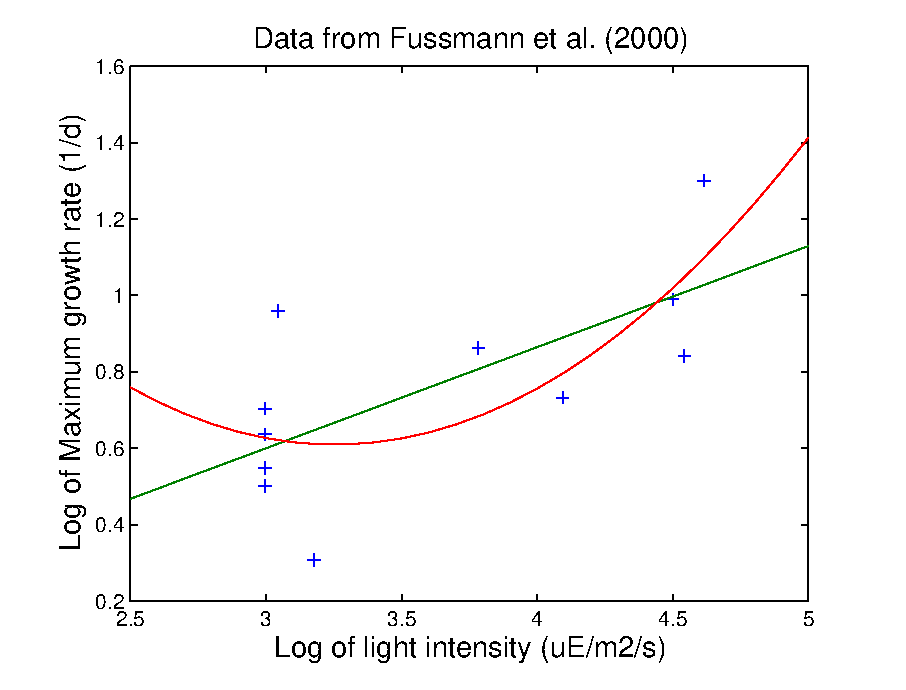
\includegraphics[width=4in]{figures/MatlabIntro2b.eps}}
\caption{Linear and quadratic regression of log growth rate on log light
intensity.} 
\label{fig2}
\end{figure}

The following exercises explore some MATLAB plotting commands. 

\textbf{Exercise\exnumber} Write an m-file that computes values $y=mx + b$
where $m =2$ and $b=2.5$ for $x$ = 1 through 10, and plots $y$ versus $x$ 
as a solid curve (in this case, a line). Recall that 
\ttt{x=1:10} creates x as a vector of the integers from 1 to 10. 

\textbf{Exercise\exnumber}. It is possible to place several plots together in one figure 
with the subplot command. \\
\tab \ttt{subplot(m,n,p)} \\
divides the figure into $m$ rows and $n$ columns. $p$ specifies which of the $mn$ plots is to be
used. More information can be obtained with \texttt{>> help subplot}. \\
Save Intro2.m with a new name and modify the program as
follows. Plot rmax as a function of Light, and log(rmax) as a function of log(Light) in 
the same figure by inserting the commands\\
\tab  \ttt{subplot(2,1,1)}  and   \ttt{subplot(2,1,2)}\\
immediately before the corresponding plot commands, so that both plots are stacked
in a single column. 

\textbf{Exercise\exnumber} Matlab automatically scales the x and y axis in plots. 
You can control the scaling using the axis command.  The command\\
\tab \ttt{axis('equal')} \\
\textbf{after} the plot command forces Matlab to use the same scale on both axes. 
The axis command can also be used to zoom in or out by setting 
the minimum and maximum values for the x and y axes. Create another plot of rmax vs. Light 
using the command \\ \tab \ttt{axis([15 105 1  4])} \\ to zoom in.

\section{Vectors}
\vspace{-0.15in} 
MATLAB uses vectors and matrices (1- and 2-dimensional rectangular arrays of 
numbers) as its primary data types. Operations with vectors and matrices may 
seem a bit abstract, but we need them to do useful things later. 

We've already seen two ways to create vectors in Matlab: \\
(1) a command or line in an m-file listing the values, like \\ 
\tab \ttt{>> initialsize=[1,3,5,7,9,11]} 

(2) using the load command, as in\\ 
\tab \ttt{>> initialsize=load('c:$\backslash \backslash $matlab6p1$\backslash 
\backslash $work$\backslash \backslash $initialdata.txt')} \\ 
(Note: if the file you're trying to load doesn't exist, this won't work!
You can also use the \textbf{open} button on the File menu instead of the command 
\ttt{>> load} to load the file into the Matlab workspace.) 

Once a vector has been created it can be used in calculations as if it were 
a number (more or less) 
\begin{verbatim}
>>finalsize=initialsize+1 
finalsize=
    2 4 6 8 10 12
>> newsize=sqrt(initialsize)
newsize = 
    1.0000 1.7321 2.2361 2.6458 3.0000 3.3166
\end{verbatim} 
Notice that the operations were applied to every entry in the vector. 
Similarly, \\
\tab \ttt{initialsize-5, 2*initialsize, initialsize/10} \\
apply subtraction, multiplication, and division to each element of the 
vector. But now try

\tab \ttt{>> initialsize$\wedge$2}

and MATLAB responds with
\begin{verbatim}
??? Error using ==> ^
Matrix must be square.
\end{verbatim} 

Why? Because \ttt{initialsize$\wedge$2} is interpreted as initialsize*initialsize, and 
$*$ indicates \textbf{matrix multiplication}. It was OK to compute 
2*initialsize because Matlab interprets multiplication with a $1 \times 1$ matrix
as scalar multiplication. But matrix multiplication of \textbf{A*A} is only 
possible if \textbf{A} is a square matrix (number of rows equal to the 
number of columns). 

Entry-by-entry operations are indicated by a period before the 
operation symbol:
\begin{verbatim}
    >> nextsize=initialsize.^2
    >> x=initialsize.*newsize
    >> x=initialsize./finalsize
\end{verbatim}
Note that addition and subtraction are always term-by-term.

\subsection*{Functions for vector construction}
\vspace{-0.15in} 
A set of regularly spaced values can be constructed by \\
\tab \textbf{x=start:increment:end} 
\begin{verbatim} 
>> x=0:1:10
x =
     0 1 2 3 4 5 6 7 8 9 10
\end{verbatim} 
The increment can be positive or negative. If you omit the increment it is 
assumed to be 1, hence \texttt{x=0:10} gives the same result as 
\texttt{x=0:1:10}. 

\texttt{x=linspace(start, end, length) }lets you specify the number of steps 
rather than the increment.
\begin{verbatim}
>> x=linspace(0,10,5)
x =
         0    2.5000    5.0000    7.5000   10.0000
\end{verbatim} 
Note that \texttt{linspace} requires commas as the separators, instead of 
colons.

\textbf{Exercise\exnumber} Create a vector v=[1 5 9 13], first using the 
\texttt{v=a:b:c} construction, and then using 
\texttt{v=linspace(a,b,c)}. 

\textbf{Exercise\exnumber} The sum of the geometric series $1 + r + r^2 + r^3 + ... + r^n$ 
approaches the limit $1/(1-r)$ for $r < 1$ as $n \rightarrow \infty$.   
Take $r=0.5$ and $n=10$, and write a \textbf{one-statement} command that creates 
the vector $[r^0, r^1, r^2, \ldots , r^n]$ and computes the sum of all its elements. 
Compare the sum of this vector to the limiting value $1/(1-r)$. Repeat this for  
$n=50$.

\subsection*{Vector addressing} 
\vspace{-0.15in} 
Often it is necessary to extract a specific 
entry or other part of a vector. This is done using subscripts, for example:
\begin{verbatim}
>> initialsize(3)
ans =
     5
\end{verbatim}
This extracts the third element in the vector. You can also access a block 
of elements using the functions for vector construction
\begin{verbatim}
c=initialsize(2:5)
c =
     3    5    7    9
\end{verbatim}
This has extracted the 2$^{nd}$ through 5$^{th}$ elements in the vector. If you 
type in \\
\tab \ttt{>> c=initialsize(4:2:6)} \\
the values in parentheses are interpreted as in vector creation 
\texttt{x=(a:b:c)}. So what do you think this command will do? Try it and 
see. 

Extracted parts don't have to be regularly spaced. For example
\begin{verbatim}
>> c=initialsize([1 2 5])
c =
     1    3    9
\end{verbatim}
extracts the 1$^{st}$, 2$^{nd}$, and 5$^{th}$ elements. 

Addressing is also used to \textbf{set specific values within a vector}. For 
example, \\
\tab \ttt{>> initialsize(1)=12}\\
changes the value of the first entry in initialsize while leaving the rest 
alone, and \\
\tab \ttt{>> initialsize([1 3 5])=[22 33 44]}
changes the 1$^{st}$, 3$^{rd}$, and 5$^{th}$ values. 

\textbf{Exercise\exnumber} Write a \textbf{one-line} command to extract 
the the second, first, and third elements of initialsize \textbf{in that 
order}. 

\subsection*{Vector orientation} 
\vspace{-0.15in} 
We will also need column vectors. A vector 
is entered as a column by using semi-colons: 
\begin{verbatim}
>> a=[1; 2; 3]
a =
     1
     2
     3
\end{verbatim}

The transpose operator \ttt{'} changes a row vector into a column vector, and vice-versa: 

\begin{verbatim}
>> initialsize'
ans =
     1
     3
     5
     7
     9
    11
\end{verbatim}

\texttt{transpose(initialsize)} has the same effect. 

\section{Matrices}
\vspace{-0.15in} 
A matrix is a two-dimensional array of numbers. Matrices are 
entered as if they were a column vector whose entries are row 
vectors. For example:
\begin{verbatim}
>> A=[1 2 3; 4 5 6; 7 8 9]
A =
     1     2     3
     4     5     6
     7     8     9
\end{verbatim}
The values making up a row are entered with white space or commas between 
them. A semicolon indicates the end of one row and the start of the next 
one. The same process lets you combine vectors to make matrices. For example 

\tab \texttt{>> L=1:3; W=2*L; B=[L;W;L]} 

creates \ttt{B} as a 3-row matrix whose $1^{st}$ and $3^{rd}$ rows are L=[1 2 3] and the 
$2^{nd}$ row is W=[2 4 6]. Similarly \\
\tab \texttt{>> C=[A, B] } or \\
\tab \texttt{>> C=[A B] } \\
creates a matrix with 3 rows and 6 columns. As with vector creation, 
the comma between entries is optional. 

MATLAB has many functions for creating and working
with matrices (Table \ref{MatrixFunctions}; 
Uniform(0,1) means that all values between 0 and 1 are equally 
likely; Normal(0,1) means the bell-shaped Normal (also called Gaussian) 
distribution with mean 0, standard deviation 1). 

\begin{table}
\begin{tabular}{p{140pt}p{280pt}}
\hline \hline
{\tt zeros(n,m)} & $n \times m$ matrix of zeros  \\
{\tt ones(n,m)} & $n \times m$ matrix of ones  \\
{\tt rand(n,m)} & $n \times m$ matrix of Uniform(0,1) random numbers \\
{\tt randn(n,m)} & $n \times m$ matrix of Normal($\mu=0,\sigma=1$) random numbers \\
{\tt eye(n)} & $n \times n$ identity matrix \\
{\tt diag(v)} & diagonal matrix with vector \ttt{v} as its diagonal \\
{\tt linspace(a,b,n)} & vector of n evenly spaced points running from a to b \\
{\tt length(v)} & length of vector v \\
{\tt size(A)} & dimensions of matrix A [\# rows, \# columns] \\
{\tt find(A)} & locate indices of nonzero entries in A \\
{\tt min(A), max(A), sum(A)} & minimum, maximum, and sum of entries \\
\hline \hline
\end{tabular}
\caption{Some important functions for creating and working with vectors and matrices; many more
are listed in the Help system, Functions by Category:Mathematics:Arrays and Matrices. Many
of these functions have additional optional arguments; use the Help system for full details.}
\label{MatrixFunctions}
\end{table}

\subsection*{Matrix addressing}
\vspace{-0.15in}  
Matrix addressing works like vector addressing except that you have 
to specify both row and column, or a range of rows and columns. For 
example \texttt{q=A(2,3)} sets q equal to 6, which is the (2$^{nd}$ row, 
3$^{rd}$ column) entry of the matrix \textbf{A}, and 

\begin{verbatim}
>> v=A(2,2:3)
v =
     5     6
>> B=A(2:3,1:2)
B =
     4     5
     7     8
\end{verbatim} 
The Matlab Workspace shows that \texttt{v} is a row vector (i.e. 
the orientation of the values has been preserved) and \texttt{B} is a 
2$\times$2 matrix. 

There is a useful shortcut to extract entire rows or columns, a colon with 
the limits omitted
\begin{verbatim}
>> firstrow=A(1,:)
firstrow =
     1     2     3
\end{verbatim}
The colon is interpreted as ``all of them", so for example \texttt{A(3,:)} 
extracts all entries in the $3^{rd}$ row, and \texttt{A(:,3)}extracts 
everything in the $3^{rd}$ column of A. 

As with vectors, addressing works in reverse to assign values to matrix 
entries. For example,
\begin{verbatim}
>> A(1,1)=12
A =
    12     2     3
     4     5     6
     7     8     9
\end{verbatim}
The same can be done with blocks, rows, or columns, for example
\begin{verbatim}
A(1,:)=rand(1,3)
A =
    0.9501    0.2311    0.6068
    4.0000    5.0000    6.0000
    7.0000    8.0000    9.0000
\end{verbatim} 
A numerical function applied to a matrix acts element-by-element: 
\begin{verbatim}
>> A=[1 4; 9 16]; A, sqrt(A)
A =
     1     4
     9    16
ans =
     1     2
     3     4
\end{verbatim}
The same is true for scalar multiplication and division. Try 

\tab \texttt{>> 2*A, A/3} 

and see what you get. 

If two matrices are the same size, then you can do element-by-element 
addition, subtraction, multiplication, division, and exponentiation:  

\tab \texttt{A+B, A-B, A.*B, A./B, A.$\wedge$B} 

\textbf{Exercise\exnumber} Use \texttt{rand} to construct a 5$\times $5 
matrix of random numbers with a uniform distribution on $[0,1]$, and then (a) Extract 
from it the second row, the second column, and the 3$\times $3 matrix of the 
values that are not at the margins (i.e. not in the first or last row, or 
first or last column). (b) Use \texttt{linspace} to replace the values in the first row by 
\texttt{2 5 8 11 14. }

\section{Iteration (``Looping")}
\vspace{-0.15in}  
Loops make it easy to do the same operation over and over again, for 
example: 
\begin{itemize}
\item make population forecasts 1 year ahead, then 2 years ahead, then 3, {\ldots}
\item update the state of every neuron based on the inputs it received in the last time interval. 
\end{itemize}
There are two kinds of loops in Matlab: \textbf{for} loops, and 
\textbf{while} loops. A \textbf{for} loop runs for a specified number of 
steps. These are written as
\begin{verbatim} 
for x=vector;
    commands
end;
\end{verbatim} 
(The semicolons after the \ttt{for} and \ttt{end} lines are optional; some other
programming languages require them, so some of us write Matlab that way too).  

Here's an example (in \textbf{Loop1.m}): 
\begin{verbatim}
% initial population size
initsize=4; 

% create matrix to hold results sizes and store initial size 
popsize=zeros(10,1); popsize(1)=initsize;

% calculate population size at times 2 through 10, write to Command Window
for n=2:10;  
      popsize(n)=popsize(n-1)*2;
      x=log(popsize(n));
      q=[num2str(n), '  ', num2str(x)];
      disp(q)
end; 
\end{verbatim}

The first time through the loop, $n$=2. The second time through, $n$=3. When it 
reaches n=10, the loop ends and the program starts executing commands that 
occur after the end statement. The result is a table of the log population 
size in generations 2 through 10. [Note also the commands for displaying the 
results. The \texttt{num2str} function converts numbers into ``strings" -- 
sequences of characters; then we put them together with some white space 
into a row vector \texttt{q}, and the \texttt{disp} function writes it out 
to the Command window]. 

Loops can be nested within each other. In the example below 
(\textbf{Loop2.m}), notice that the second loop is \textbf{completely} 
inside the first. Loops must be either \textbf{nested} (one completely 
inside the other) or \textbf{sequential} (one starts after the previous one 
ends). 
\begin{verbatim}
p=zeros(5,1);					            
for init=linspace(1,10,3);			
	p(1)=init; 				            
	for n=2:5;					        	
          p(n)=p(n-1)*2; x=log(p(n));		  
          q=[num2str(n), '  ', num2str(x)];	
          disp(q)				
      end;					           
end;						            
\end{verbatim} 

\begin{itemize}
\item Line 1 creates the vector p.
\item Line 2 starts a loop over initial population sizes
\item Lines 3-8 now do the same ``population growth" simulation as above
\item Line 9 then ends the loop over initial sizes
\end{itemize}
The result when you run \textbf{Loop2.m} is that the ``population growth" 
calculation is done repeatedly, for a series of values of the initial 
population size. To make the output a bit nicer, we can first do the 
calculations and then print them out in a second loop -- see 
\textbf{Loop3.m}. 

\textbf{Exercise\exnumber:} Imagine that while doing fieldwork in some 
distant land you and your assistant have picked up a parasite that grows 
exponentially until treated. Your case is more severe than your assistant's: 
on return to Ithaca there are 400 of them in you, and only 120 in your 
assistant. However, your field-hardened immune system is more effective. In 
your body the number of parasites grows by 10 percent each day, while in 
your assistant's it increases by 20 percent each day. That is, $j$ days after 
your return to Ithaca your parasite load is $n(j) = 400(1.1)^j$ and 
the number in your assistant is $m(j) = 120(1.2)^j$. 

Write an m-file \textbf{Parasite1.m} that uses a for-loop to compute the 
number of parasites in your body and your assistant's over the next 30 days, 
and draws a single plot of both on log-scale -- i.e. $log(n(j))$ and $log(m(j))$ 
versus time for 30 days. 

\textbf{Exercise\exnumber:} Write an m-file that uses for-loops to create the 
following 5$\times $5 matrix A. \underline{Think first:} do you want to use
nested loops, or sequential? 
\[
{\begin{array}{*{20}c}
 1 \hfill & 2 \hfill & 3 \hfill & 4 \hfill & 5 \hfill \\
 {0.1} \hfill & 0 \hfill & 0 \hfill & 0 \hfill & 0 \hfill \\
 0 \hfill & {0.2} \hfill & 0 \hfill & 0 \hfill & 0 \hfill \\
 0 \hfill & 0 \hfill & {0.3} \hfill & 0 \hfill & 0 \hfill \\
 0 \hfill & 0 \hfill & 0 \hfill & {0.4} \hfill & 0 \hfill \\
\end{array} }
\]
(Challenge: this could be done using a single for-loop. How?) 

\textbf{Exercise\exnumber} Modify {\bf Parasite1.m} so that $n(t)$ and
$m(t)$ are computed for 30 days by using vectorized computations rather
than  by looping. That is, after setting up appropriate vectors, there should
be a single statement \\
\tab {\tt n = matlab formula;} \\
in which all 30 values of $n(t)$ are computed as a vector,
followed by another statement in which all 30 values of $m(t)$ are
computed as a vector. 

\subsection*{While-loops} 
\vspace{-0.15in}  
A while-loop lets an iteration stop or continue based on whether or not
some condition holds, rather than continuing for a fixed number of iterations.  
For example, we can compute the solutions of a model until the time when some variable reaches 
a threshold value. The format of a while-loop is
\begin{verbatim}
while(condition);
    commands
end;
\end{verbatim}
The loop repeats as long as the condition remains true. \textbf{Loop4.m} 
contains an example similar to the for-loop example; run it and you will get a 
graph of population sizes over time. 

A few things to notice about the program: 
\begin{enumerate}
\item First, even though the condition in the while statement said \\
\tab \ttt{while(popsize$<$1000)}  \\
the last population value was $>1000$. That's because the condition is 
checked \textit{before} the commands in the loop are executed. When the 
population size was 640 in generation 6, the condition was satisfied so the 
commands were executed again. After that the population size is 1280, so the 
loop is finished and the program moves on to statements following the loop. 

\item Since we don't know in advance how many iterations are needed, we 
couldn't create in advance a vector to hold the results. Instead, a vector 
of results was constructed by starting with the initial population size and 
appending each new value as it was calculated. 

\item When the loop ends and we want to plot the results, the ``y-values" are 
popsize, and the x values need to be x=0:something. To find ``something", the 
\textbf{size} function is used to find the number of rows in popsize, and 
then construct an x-vector of the right size. 
\end{enumerate} 

\begin{table}
\begin{center}
\begin{tabular}{p{80pt}p{120pt}}
\hline \hline 
{\tt == } & Equal to  \\
$ {\tt \sim =}$ & Not equal to  \\
{\tt <} & Less than  \\
{\tt <=} & Less than or equal to \\
{\tt >} & Greater than \\
{\tt >=} & Greater than or equal to \\
\& & AND  \\
${\tt \vert}$ & OR \\
${\tt \sim}$ & NOT \\
\hline \hline 
\end{tabular}
\caption{Comparison and logical operators in Matlab.}
\label{LogicalOperators}
\end{center}
\end{table}

The conditions controlling a \textbf{while} loop are built up from operators 
that compare two variables (Table \ref{LogicalOperators}). Comparison operators
produce a value 1 for true statements, and 0 for false. For 
example try\\
\tab \ttt{>> a=1; b=3; c=a$<$b, d=(a$>$b)} \\
The parentheses around (a$>$b) are optional but improve readability. 

More complicated conditions are built by using the \textbf{logical operators} AND,
OR, and NOT to combine comparisons.
The OR is \textbf{non-exclusive}, meaning that x$\vert $y is true if one or 
both of x and y are true. For example:

\tab \ttt{>> a=[1,2,3,4]; b=[1,1,5,5]; (a$<$b){\&}(a$>$3), (a$<$b)$\vert $(a$>$3)}

When we compare two matrices of the same size, or compare a 
number with a matrix, comparisons are done element-by-element and the result 
is a matrix of the same size. For example
\begin{verbatim}
>> a=[1,2,3,4]; b=[1,1,5,5]; c=(a<=b), d=(b>3)
c =
     1     0     1     1
d =
     0     0     1     1
\end{verbatim}

Within a while-loop it is often helpful to have a \textbf{counter} variable
that keeps track of how many times the loop has been executed. 
In the following code, the counter variable is \texttt{n}: 
\begin{verbatim}
n=1; 
while(condition);
    commands
    n=n+1; 	
end;
\end{verbatim}
The result is that \texttt{n=1} holds while the \texttt{commands} (whatever they are)
are being executed for the first time. Afterward \texttt{n} is set to 2, which holds
during the second time that the commands are executed, and so on. This is helpful,
for example, if you want to store a series of results in a vector or matrix. 

\textbf{Exercise\exnumber} Write an m-file \textbf{Parasite2.m} that uses 
a while-loop to compute the number of parasites in your body and your 
assistant's so long as you are sicker than your assistant, and stops when your assistant 
is sicker than you. 

\section{Branching}
\vspace{-0.15in} 
Logical conditions also allow the rules for ``what happens next" in a model 
to be affected by the current values of state variables. The \texttt{if} 
statement lets us do this; the basic format is 
\begin{verbatim}
if(condition);
    commands
else;
    other commands 
end;
\end{verbatim}

If the ``else" is to do nothing, you can leave it out:
\begin{verbatim}
if(condition);
    commands
end; 
\end{verbatim}
Look at and run \textbf{a copy of} \textbf{Branch1.m} to see an \textbf{if} 
statement in action, so that the growth rate in the next time step depends 
on the current population size. You can set \textbf{breakpoints} for running the 
script by clicking on the $-$ next to the line number of a statement in the Editor 
window. This will cause Matlab to pause before it executes this statement. Once paused, 
you can step through the script line by line using the step icon at the top of the 
Editor window. 

More complicated decisions can be built up using \texttt{elseif}. 
The basic format for that is 
\begin{verbatim}
if(condition);
   commands
elseif(condition);
   other commands
else;
other commands
end; 
\end{verbatim}

\textbf{Branch2.m} uses \texttt{elseif} to have population growth tail off 
in several steps as the population size increases: 
\begin{verbatim}
if(popnow<250);
    popnow=popnow*2;
elseif (popnow<500);
   popnow=popnow*1.5;
else; 
popnow=popnow*0.95
end;
\end{verbatim}

What does this accomplish? First, if popnow is still $<$250, then growth by 
a factor of 2 occurs. Since the \texttt{if} condition was satisfied, the 
\texttt{elseif} isn't looked at; MATLAB jumps to the \texttt{end} and 
continues from there. If popnow is not $<$250, MATLAB moves on to the 
\texttt{elseif}. If popnow is $<$500 the growth factor of 1.5 applies, and 
MATLAB then jumps to the \textbf{end} and continues from there. If not, the 
final \texttt{else} block is executed and population declines by 5{\%} 
instead of growing. 

\textbf{Advanced flow control:} Matlab has some additional statements that can be used to control 
which statements in a program are executed: 
\begin{itemize}
\item \textbf{switch} allows the value of a variable to
decide which one, among several code blocks, is executed.
\item \textbf{continue} causes a for or while loop to skip over any
remaining statements until the end of the loop, and then make the
next iteration of the loop.
\item \textbf{break} terminates immediately the execution of a loop. The program
then jumps to the first statement after the \texttt{end} of the loop
\end{itemize}  
We won't be using these in these notes, but they might come in handy for your own work. 
For detailed descriptions of these and more see the Help System,  
\textbf{Programming and Data Types: M-File Programming: Flow Control}.

\textbf{Exercise\exnumber} Modify \textbf{Parasite1.m} so 
that there is random variation in parasite success, depending on whether
or not conditions on a given day are stressful. Specifically, on ``bad days'' the parasites increase
by 10\% while on ``good days'' they are beaten down by your immune system and they go 
down by 10\%, and similarly for your assistant. That is, 
\begin{equation*}
\begin{aligned}
\mbox{Bad days:  }  & n(j+1)=1.1n(j), & m(j+1)=1.2m(j) \hfill \\
\mbox{Good days: }  & n(j+1)=0.9n(j), & m(j)=0.8m(j) \hfill \\
\end{aligned}
\end{equation*} 
Do this by using \texttt{rand(1)} and an \texttt{if} statement
to ``toss a coin'' each day: if the random value produced by \texttt{rand} for
that day is $<0.35$ it's a good day, and otherwise it's bad. 

\section{Matrix computations} \label{MatComp} 
\vspace{-0.15in} 
One of Matlab's strengths is its suite of functions for matrix  
calculations. Some functions that we will eventually find useful are 
listed in Table \ref{MatrixComputationsTable}; don't panic if you don't
know what these are -- they'll be defined when we use them. 

\begin{table}
\begin{tabular}{p{120pt}p{300pt}}
\hline \hline 
{\tt inv(A)} & inverse of matrix A  \\
{\tt det(A)} & determinant of matrix A  \\
{\tt trace(A)} & trace of matrix A \\
{\tt poly(A)} & coefficients of characteristic polynomial \\
{\tt expm(A)} & matrix exponential \\
{\tt norm(A)} & Euclidean matrix norm  \\
{\tt find(A)} & locate indices and values of nonzero entries \\
{\tt v=eig(A)} & vector of the eigenvalues of A, unsorted \\
{\tt [W,D]=eig(A)} & diagonal matrix D of eigenvalues; matrix W whose columns are the corresponding eigenvectors \\
\hline \hline 
\end{tabular}
\caption{Some important functions for matrix computations. Many
of these functions have additional optional arguments; use the Help system for full details.}
\label{MatrixComputationsTable}
\end{table}

Many of these functions only work on square matrices, and return an error if \ttt{A} is not square. 
\textbf{For the remainder of this section we only consider square matrices}, and focus on functions for 
finding their eigenvalues and eigenvectors.

We are often particularly interested in the dominant eigenvalue -- the one with 
largest absolute value -- and the corresponding eigenvector (the general 
definition of absolute value, which covers both real and complex numbers, is 
$\left| {a + bi} \right| = \sqrt {a^2 + b^2} )$. Extracting those from the 
complete set produced by \textbf{eig} takes some work. For
the dominant eigenvalue: 
\begin{verbatim}
    >> A=[5 1 1; 1 -3 1; 0 1 3]; L=eig(A); 
    >> j=find(abs(L)==max(abs(L)))
    >> L1=L(j);
    >> ndom=length(L1);
\end{verbatim}

In the second line \texttt{abs(L)==max(abs(L))} is a comparison 
between two vectors, which returns a vector of 0s and 1s. 
Then \textbf{find} extracts the list of indices where the 1's are. 

The third line uses the ``found" indices to extract the dominant 
eigenvalues. Finally, \texttt{length} tells us how many entries there are in \texttt{L1}. 
If ndom=1, there is a single dominant eigenvalue $\lambda $. 

The \textbf{dominant eigenvector(s)} are also a bit of work. 
\begin{verbatim}
>> [W,D]=eig(A)
>> L=diag(D)
>> j=find(abs(L)==max(abs(L)));
>> L1=L(j); 
>> w=W(:,j); 
\end{verbatim}

The first line supplies the raw ingredients, and the second pulls
the eigenvalues from D into a vector. After that it's the
same as before. The last line constructs a matrix with dominant
eigenvectors as its columns. If there is a single dominant eigenvalue, then \texttt{L1} 
will be a single number and \texttt{w} will be a column vector. 

To get the corresponding \textbf{left eigenvector(s)}, repeat the whole 
process on \texttt{\textbf{B=transpose(A). }}

\subsection*{Eigenvector scalings}
\vspace{-0.15in}
The eigenvectors of a matrix population model have biologically meanings
that are clearest when the vectors are suitably scaled. 
The dominant right eigenvector \textbf{w} is 
the stable stage distribution, and we are most interested in the relative 
proportions in each stage. To get those, 

\tab \texttt{>> w=w/sum(w);}

The dominant left eigenvector \textbf{v} is the reproductive value, and it 
is conventional to scale those relative to the reproductive value of a 
newborn. If newborns are class 1: \\
\tab \texttt{>> v=v/v(1);}

\textbf{Exercise\exnumber}: Write an m-file which applies the above to 
A=[1 5 0; 6 4 0; 0 1 2]. Your file should
first find \textbf{all} the eigenvalues of A, then extract the dominant one and the 
corresponding (right) eigenvector, scaled as above. Repeat this for the transpose
of A to find the dominant left eigenvector, scaled as above.  

\subsection{Eigenvalue sensitivities and elasticities}
\vspace{-0.15in}
For an $n\times n$ matrix \texttt{A} with entries $a_{ij}$, the sensitivities 
$s_{ij} $ and elasticities $e_{ij} $ can be computed as
\begin{equation}
\label{eq1}
s_{ij} = \frac{\partial \lambda }{\partial a_{ij} } = \frac{v_i w_j 
}{\left\langle {v,w} \right\rangle }\quad \quad e_{ij} = \frac{a_{ij} 
}{\lambda }s_{ij} 
\end{equation}
where $\lambda $ is the dominant eigenvalue, \textbf{v} and \textbf{w} are 
dominant left and right eigenvalues, and $\left\langle {v,w} \right\rangle $ 
is the inner product of \textbf{v} and \textbf{w}, computed in Matlab as 
\texttt{dot(v,w)}. So once $\lambda, v, w$ have been 
found and stored as variables, it just takes some for-loops to compute the 
sensitivities and elasticities.
\begin{verbatim}
n=length(v); 
vdotw=dot(v,w); 
for i=1:n; for j=1:n;
    s(i,j)=v(i)*w(j)/vdotw;
end; end;
e=(s.*A)/lambda;
\end{verbatim}

Note how the elasticities are computed all at once in the last line. In 
Matlab that kind of ``vectorized" calculation is \textbf{much} quicker than 
computing them one-by-one in a loop. Even faster is turning the loops
into a matrix multiplication: 
\begin{verbatim}
vdotw=dot(v,w); 
s=v*w'/vdotw;
e=(s.*A)/lambda;
\end{verbatim}

\textbf{Exercise\exnumber} Construct the transition matrix \textbf{A}, 
and then find $\lambda, v, w$ for an age-structured model 
with the following survival and fecundity parameters: 
\begin{itemize}
\item  Age-classes 1-6 are genuine age classes with survival probabilities
$$(p_1, p_2, \cdots, p_6 ) = (0.3, 0.4, 0.5, 0.6, 0.6, 0.7)$$
Note that $p_j = a_{j + 1,j}$, the chance of surviving from age $j$ to age 
$j+1$, for these ages. You can create a vector \ttt{p} with the 
values above and then use a for-loop to put those values into 
the right places in \ttt{A}. 
\item Age-class 7 are adults, with survival 0.9 and fecundity 12. 
\end{itemize} 

\textbf{Results}: $\lambda =1.0419$
\[
A = \left( {\begin{array}{*{20}c}
   0 & 0 & 0 & 0 & 0 & 0 & {12}  \\
   {.3} & 0 & 0 & 0 & 0 & 0 & 0  \\
   0 & {.4} & 0 & 0 & 0 & 0 & 0  \\
   0 & 0 & {.5} & 0 & 0 & 0 & 0  \\
   0 & 0 & 0 & {.6} & 0 & 0 & 0  \\
   0 & 0 & 0 & 0 & {.6} & 0 & 0  \\
   0 & 0 & 0 & 0 & 0 & {.7} & {.9}  \\

 \end{array} } \right)
\]
$w = (0.6303,0.1815,0.0697,0.0334,0.0193,0.0111)$ \\
$v = (1,3.4729,9.0457,18.8487,32.7295,56.8328,84.5886)$ \\

\section{Creating new functions}
M-files can be used to create new functions, which then can be used in the 
same way as Matlab's built-in functions. Function m-files are often 
\textbf{useful} because they let you break a big program into a series of 
steps that can be written and tested one at a time. They are also sometimes 
\textbf{necessary}. For example, to solve a system of differential equations 
in Matlab, you have to write a function m-file that calculates the rate of change 
for each state variable. 

\subsection{Simple functions}  
Function m-files have a special format. Here 
is an example, \texttt{mysum.m} that calculates the sum of the entries in a 
matrix [the \texttt{sum} function applied to a matrix calculates the sum of 
each column, and then a second application of \texttt{sum} gives the sum of 
all column sums]. 
\begin{verbatim}
function f=mysum(A);
    f=sum(sum(A));
return;
\end{verbatim} 
This example illustrates the rules for writing function m-files: 
\begin{enumerate}
\item The first line must begin with the word \texttt{function}, followed by an 
expression of the form: \texttt{variable\_name = function\_name(function arguments)} 
\item The function name \textbf{must} be the same as the name of the m-file. 
\item The last line of the file is \texttt{return;} (this is not required in the 
current version of Matlab, but is useful for compatibility with older versions). 
\item In between are commands that calculate the function value, and assign it to the 
variable \texttt{variable\_name} that appeared in the first line of the function. 
\end{enumerate}

In addition, the function m-file must be in a folder that's on Matlab's 
search path. You can put it in a folder that's automatically part of the 
search path such as Matlab's \texttt{work} folder, or else use the 
\texttt{addpath} command to augment the search path. 

Matlab gives you some help with these rules. When you create an m-file using 
\textbf{File/New/M-file} on the Matlab toolbar, Matlab's default is to save 
it under the right name in the \texttt{work} folder. If everything is done 
properly, then \texttt{mysum} can be used exactly like any other Matlab 
function. 
\begin{verbatim}
>> mysum([1 2])
ans =
	3
\end{verbatim} 

\subsection{Functions with multiple arguments or returns}
Matlab functions can have more than one argument, and can return more than one calculated 
variable. The function \textbf{eulot.m} is an example with multiple arguments. It computers the 
Euler-Lotka sum $$\sum\limits_{a=0}^n {\lambda ^{-(a+1)}l_a f_a -1}$$ as a 
function of $\lambda$, and vectors containing the values of $l_a$ and $f_a.$ 
\begin{verbatim}
function f=eulot(lambda,la,fa);
    age=0:(length(la)-1);
    y=lambda.^(-(age+1));
    f=sum(y.*la.*fa)-1;
return;
\end{verbatim} 
We have seen that (given the values of $l_a$ and $f_a$) the dominant 
eigenvalue $\lambda$ of the age-structured model results in this expression 
equaling 0. Type in \\
\tab \ttt{>> la=[0.9 0.8 0.7 0.5 0.2]; fa=[0 0 2 3 5];} \\
and then you should find that \texttt{eulot(1.4,la,fa)} and 
\texttt{eulot(1.5,la,fa)} have opposite signs, indicating that $\lambda$ is 
between 1.4 and 1.5. 

To have more than one returned value, the first line in the m-file is slightly different: 
the various quantities to be returned are enclosed in [ ]. An example is 
\textbf{stats.m}: 
\begin{verbatim}
function [mean_x,var_x,median_x,min_x,max_x]=stats(x); 
    mean_x=mean(x); var_x=var(x); 
    median_x=median(x);
    min_x=min(x); max_x=max(x);
return;
\end{verbatim} 

Function m-files can contain \textit{subfunctions}, which are functions called by the main function (the one whose name appears in the m-file name). Subfunctions are ``visible'' only within the m-file where they are defined. In particular, you cannot call a subfunction at the Command line, or in another m-file. 
For example, create an m-file \texttt{Sumgeseries.m} with the following commands:  
\begin{verbatim}
function f=Sumgseries(r,n);
    u=gseries(r,n); f=sum(u);
return; 
function f=gseries(r,n);
   f=r.^(0:n); 
return;
\end{verbatim}
Only the first of the two functions -- the one with the same name as the m-file 
will be 'visible' to Matlab. That is: 
\begin{verbatim}
>> Sumgseries(0.1,500)
ans =
    1.1111
>> gseries(0.1,500)
??? Undefined command/function 'gseries'.
\end{verbatim}

\textbf{Exercise\exnumber} Use \ttt{z=randn(500,1)} to create a matrix of 500 Gaussian 
random numbers. Then try \ttt{a=stats(z)}, \ttt{[a,b]=stats(z)}, and \ttt{[a,b,c]=stats(z)}
to see what Matlab does if you ``ask for" a smaller number of 
returned values than a function computes. Remember, you'll have to put a copy of \texttt{stats.m}
into a folder on your search path. 

\textbf{Exercise\exnumber} Modify \ttt{stats.m} so that it also returns the
value of \ttt{srsum(x)} where the function \ttt{srsum(x)=sum(sqrt(x))} is defined using
a subfunction rather than within the body of \ttt{stats}. When that's working,
try \ttt{srsum([1 2 3])} at the Command line and see what happens. 

\textbf{Exercise\exnumber}. Write a function m-file \texttt{rmatrix.m} 
which takes as arguments 3 matrices $A,S,Z$, and 
returns the matrix $B=A+S.*Z$. When it's working you should be able to 
do: 
\begin{verbatim}
>> A=ones(2,2); S=0.5*eye(2); Z=ones(2,2); B=rmatrix(A,S,Z)
B =
    1.5000    1.0000
    1.0000    1.5000
\end{verbatim} 

\section{A simulation project}
This section is an optional ``capstone'' project putting into use the  
Matlab programming skills that have been covered so far. Nothing new about
Matlab \textit{per se} is covered in this section.  

The first step is to write a script file that simulates a simple model for density-independent 
population growth with spatial variation. The model is as follows. The \textit{state variables}  
are the numbers of individuals in a series of $L = 20$ 
patches along a line ($L$ stands for ``length of the habitat") . 
\begin{table}
\begin{tabular}
{|p{22pt}|p{22pt}|p{22pt}|p{22pt}|p{22pt}|p{22pt}|p{22pt}|p{22pt}|p{22pt}|p{22pt}|p{22pt}|p{22pt}|}
\hline
1& 
2& 
3& 
4& 
... & 
& 
& 
& 
& 
...& 
L-1& 
L \\
\hline
\end{tabular}
\end{table}

Let $N_j(t)$ denote the number of individuals in patch $j$ ($j=1,2,\ldots, L$) at 
time $t$ ($t=1,2,3,\ldots$ ), and let $\lambda _j$ be the geometric growth rate 
in patch $j$. The \textit{dynamic equations} for this model consist of two steps:
\begin{enumerate}
\item Geometric growth within patches: 
\begin{equation}
M_j(t) = \lambda _j N_j(t) \quad \mbox{ for all } j. 
\end{equation}
\item Dispersal between neighboring patches:
\begin{equation}
N_j(t + 1) = (1 - 2d)M_j(t) + dM_{j - 1}(t) + dM_{j + 1}(t) \quad \mbox{ for } 2 \le j \le L-1 
\label{disperse1}
\end{equation}
where $2d$ is the ``dispersal rate". We need special rules for the end patches. 
For this exercise we assume \textit{reflecting boundaries}: those who venture out 
into the void have the sense to come back. That is, there is no 
leftward dispersal out of patch 1 and no rightward dispersal out of patch $L$:
\begin{equation}
\begin{array}{l}
 N_1(t + 1) = (1 - d)M_1(t) + dM_2(t) \\ 
 N_L(t + 1) = (1 - d)M_L(t) + dM_{L - 1}(t) \\ 
\end{array}
\label{disperse2}
\end{equation}
\end{enumerate} 
$\bullet$ Write your script to \underline{start} with 5 individuals in each patch at 
time $t$=1, \underline{iterate} the model up to $t$=50, and \underline{graph} 
the log of the total population size (the sum over all patches) over time. Use the 
following growth rates: $\lambda _j = 0.9$ in the left half of the patches, 
and $\lambda _j = 1.2$ in the right. \\
$\bullet$ Write your program so that $d$ and $L$ are parameters, 
in the sense that the first line of your script file reads \texttt{d=0.1; L=20;} 
and the program would still work if these were changed other values. 

Notes and hints:
\begin{enumerate}
\item This is a real programming problem. Think first, then start writing your 
code. 
\item Notice that this model is not \textit{totally} different from \textbf{Loop1.m}, 
in that you start with a founding population at time 1, and use a loop
to compute successive populations at times 2,3,4, and so on. The difference
is that the population is described by a vector rather than a number. Therefore,
to store the population state at times $t=1,2,\cdots,50$ you will need
a matrix \ttt{njt} with 50 rows and $L$ columns. Then \ttt{njt(t,:)} is the population 
state vector at time $t$. 
\item \textbf{Vectorize!} Vector/matrix operations are \underline{much}  
faster than loops. Set up your calculations so that computing $M_j(t) = 
\lambda_j N_j(t)$ for $j=1,2,\cdots,L$ is a \texttt{one-line} statement of the form \texttt{a=b.*c }. 
Then for the dispersal step: if $M_j(t), j=1,2,\ldots,L$ is stored as a vector \ttt{mjt} of length
$L$, then what (for example) are $M_j(t)$ and $M_{j \pm 1}(t)$ for $2 \le j \le (L-1)$? 
\end{enumerate}

\textbf{Exercise\exnumber} Use the model (modified as necessary) to ask how the spatial 
arrangement of good versus bad habitat patches affects the  
population growth rate. For example, does it matter if all the good sites 
($\lambda >1$) are at one end or in the middle? What if they aren't all in 
one clump, but are spread out evenly (in some sense) across the entire 
habitat? \textbf{Be a theoretician}: (a) Patterns will be easiest to see if 
good sites and bad sites are very different from each other. (b) Patterns 
will be easiest to see if you come up with a nice way to compare growth 
rates across different spatial arrangements of patches. (c) Don't confound 
the experiment by also changing the proportion of good versus bad patches at
the same time you're changing the spatial arrangement. 

\textbf{Exercise\exnumber} Modify your script file for the model (or write
it this way to begin with...) so that the dispersal phase (equations \ref{disperse1}
and \ref{disperse2}) is done by calling a subfunction \texttt{reflecting}
whose arguments are the pre-dispersal population vector $M(t)$ and the dispersal 
parameter $d$, and which returns $N(t+1)$, the population vector after dispersal
has taken place. 

\section{Coin tossing and Markov Chains} \label{Mchain}
The exercises on coin tossing and Markov chains in Chapter 3 can be used
as the basis for a computer-lab session. For convenience we also 
include them here. All of the Matlab functions and programming methods required for these exercises 
have been covered in previous sections, but it is useful to look back and remember
\begin{itemize}
\item how to generate sets of random uniform and Gaussian random numbers using 
\texttt{rand} and \texttt{randn}.
\item how logical operators can be used to convert a vector of numbers into a vector of 1's and 0's 
according to whether or not a condition holds.
\item how to find the places in a vector where the value changes, using logicals
and \texttt{find}.
\end{itemize}  
\begin{verbatim}
>> v=rand(100,1);  
>> u = (v<0.3); 
>> w=find(u[2:100]~=u[1:99])
\end{verbatim}

\textbf{Coin tossing} 
\textbf{Exercise\exnumber} Experiment with sequences of coin flips produced by
a random number generator: 
\begin{itemize}
\item Generate a sequence \texttt{r} of 1000 random numbers uniformly
distributed in the unit interval $[0,1]$.
\item Compute and plot a histogram for the values
with ten equal bins of length 0.1. How much variation is there in values of the
histogram? Does the histogram make you suspicious that the numbers are not independent and uniformly 
distributed random numbers? 
\item Now compute sequences of 10000 and 100000 random numbers uniformly
distributed in the unit interval $[0,1]$, and a histogram for each with ten equal bins.
Are your results consistent with the prediction of the central limit theorem that the range of variation
between bins in the histogram is proportional to the square root of the sequence length?
\end{itemize}

\textbf{Exercise\exnumber} Convert the sequence of 1000 random numbers \texttt{r} from the previous 
exercise into a sequence of  outcomes of coin tosses in which the probability of heads is $0.6$
and the probability of tails is $0.4$. 
Let $1$ represent
an outcome of heads and let $0$ represent an outcome of tails.  
To generate from \texttt{r}
a sequence of $0$'s and $1$'s that reflect these
probabilities, we assign random numbers less than $0.4$ to tails, and
random numbers larger than $0.6$ to heads.  
A simple way to do this follows:
%

\begin{verbatim}
seq = zeros(1000,1);
for i=1:1000
  if r(i) < 0.6
    seq(i)=1;
  end
end
\end{verbatim}

\textbf{\underline{Matlab Challenge}} Write a ``vectorized'' program 
to generate the coin tosses without using the command \texttt{for}.

(Hint: The logical operator \texttt{<} can act on vectors and matrices
as well as scalars.)

\begin{itemize} 
\item Recall that this coin tossing experiment can be modeled by
the binomial distribution: the probability of $k$
heads in the sequence is given by 
$$c_k (0.6)^k (0.4)^{1000-k} \quad \mbox{ where } c_k=\frac{1000!}{k!(1000-k)!}.$$ 
Calculate the probability of $k$ heads for 
values of $k$ between 500 and 700 in a sequence of 1000
independent tosses.  Plot your results with $k$ on the 
$x$-axis and the probability of $k$ heads on the $y$-axis.
Comment on the shape of the plot. 
\item Now test the binomial distribution by doing 1000 repetitions of the sequence of 1000 coin tosses and plot
a histogram of the number of heads obtained in each repetition. 
Compare the results with the predictions from the binomial distribution. 
\item Repeat this experiment with 10000 repetitions of 100
coin tosses. Comment on the differences you observe between this
histogram and the histogram for 1000 repetitions of tosses of 1000 coins.
\end{itemize}

\textbf{Markov chains} 
The purpose of the following exercises is to generate synthetic data for 
single channel recordings from finite state Markov chains, and explore patterns in the data. 

Single channel recordings give the times that a Markov chain makes a transition from a closed to an open
state or vice versa. The histogram of expected residence times 
for each state in a Markov chain is exponential, with different mean residence time for different states.  
To observe this in the simplest case, we again consider coin tossing. The two outcomes, heads or
tails, are the different states in this case. Therefore the histogram of residence times for heads and tails should 
each be exponential. The following steps are taken to compute the residence times:

\begin{itemize}
\item Generate sequences of independent coin tosses based on given 
probabilities.
\item Look at the number of \emph{transitions} that occur in
each of the sequences (a \emph{transition} is when two successive tosses give different 
outcomes).
\item Calculate the residence times by counting the
number of tosses between each transition. \end{itemize}

\textbf{Exercise \exnumber} Find the script \texttt{cointoss.m}. This program calculates
the residence times of coin tosses by the above methodology. Are the residence times consistent with the prediction that 
their histogram decreases exponentially? Produce a plot that compares the predicted results with the 
simulated residence times stored by cointoss in the vectors \texttt{hhist} and \texttt{thist}.
(Suggestion: use a logarithmic scale for the values with the matlab command \texttt{semilogy}.)

Models for stochastic switching among conformational states of membrane channels are somewhat more complicated than the
coin tosses we considered above. There are usually more than 2 states, and the transition probabilities are state dependent.
Moreover, in measurements some states cannot be distinguished 
from others. We can observe transitions from an open state to a closed
state and vice versa, but transitions between open states (or between closed states)
are ``invisible''. Here we shall simulate data from a Markov
chain with 3 states, collapse that data to remove the distinction 
between 2 of the states and then analyze the data to see that it
cannot be readily modeled by a Markov chain with just two states.
We can then use the distributions of residence times for the 
observations to determine how many states we actually have.

Suppose we are interested in a membrane current that has three states:
one open state, $O$, and two closed states, $C_1$ and $C_2$. As in
the kinetic scheme discussed in class, state $C_1$ cannot make a transition
to state $O$ and vice-versa. We assume that state $C_2$ has shorter
residence times than states $C_1$ or $O$. Here is the transition
matrix of a Markov chain we will use to simulate these conditions:
\begin{eqnarray*}
&\begin{matrix}C_1&C_2&O\end{matrix}&\\
&\displaystyle{\begin{bmatrix}.98&.1&0\\
                              .02&.7&.05\\
                               0 &.2&.95\end{bmatrix}}
&\begin{matrix}C_1\\C_2\\O\end{matrix}
\end{eqnarray*}
You can see from the matrix that the probability $0.7$ of staying in
state $C_2$ is much smaller than the probability $0.98$ of staying in
state $C_1$ or the probability $0.95$ of remaining in state $O$.

\textbf{Exercise\exnumber} Generate a set of 1000000 samples
from the Markov chain with these transition probabilities. We will
label the state $C_1$ by 1, the state $C_2$ by 2 and the state $O$ by 3.
This can be done with a modification of the script we used to produce
coin tosses:
\begin{verbatim}
nt = 1000000;
A = [0.98, 0.10, 0; 0.02, 0.7, 0.05; 0, 0.2, 0.95]
sum(A)
     rd = rand(nt,1);
     states = ones(nt+1,1);
     states(1) = 3; \% Start in open state
for i=1:nt
     if rd(i) < A(3,states(i))
        states(i+1) = 3;
     elseif rd(i) < A(3,states(i))+A(2,states(i))
        states(i+1) = 2;
     end;
end;
\end{verbatim}
(If your computer does not have sufficient memory to generate 1000000 
samples, use 100000.)

\textbf{Exercise\exnumber} Compute the eigenvalues and eigenvectors of
the matrix $A$. Compute the total time that your sample data in the 
vector \texttt{states} spends in each state (try to use vector operations to do this!)
and compare the results with predictions coming from the dominant right
eigenvector of $A$.

\textbf{Exercise\exnumber} Produce a new vector \texttt{rstates}
by ``reducing'' the data in the vector 
\texttt{states} so that states 1 and 2 are indistinguishable.
The states of \texttt{rstates} will be called ``closed'' and ``open''.

\textbf{Exercise\exnumber}
Plot histograms of the residence times of the open and closed
states in \texttt{rstates} by modifying the program \texttt{cointoss.m}.  

Comment on the shapes of the distributions in each case.
Using your knowledge of the transition matrix $A$, make a prediction
about what the residence time distributions of the open states should be.
Compare this prediction with the data. Show that the residence time distribution
of the closed states is not fit well by an exponential distribution.

%\textbf{Exercise\exnumber} The histogram of expected residence times for each state in a Markov chain
%is exponential, with different exponentials for different states.  
%To observe this in the simplest case, use a random number generator
%to produce ``data'' from a two state Markov chain. Next, determine 
%the \textit{transitions} that occur as the state changes in this data, and the residence times. 
%Finally, compute histograms of the residence times for each of the two states.

\section{The Hodgkin-Huxley model}
The purpose of this section is to develop an understanding of the 
components of the Hodgkin-Huxley model for the membrane potential of
a space clamped squid giant axon. It goes with the latter part
of Chapter 3 in the text, and with the \textbf{Recommended reading:} 
Hille, Ion Channels of Excitable Membranes, Chapter 2.

The Hodgkin-Huxley model is the system of differential equations
%$$
%\displaylines{
%C \frac{dv}{dt}=i -
%\left[ {g_{Na}m^{3}h \left( {v-v_{Na}} \right) 
%+g_{K}n^{4}\left( {v-v_{K}} \right) 
%+g_{L}\left( {v-v_{L}}\right) } \right] \cr 
%\frac{dm}{dt}=3^{{{T-6.3} \over {10}}}\left[ {\left( {1-m}\right) \Psi \left( {{{-v-35} \over {10}}}
%\right) -m \left( {4 \exp \nolimits {{-v-60} \over {18}}} \right) } \right] \cr 
%\frac{dn}{dt}=3^{{{T-6.3} \over {10}}} \left[ {\left( {1-n} \right) 0.1\Psi \left( {{{-v-50} \over {10}}} \right) 
%-n\left( {0.125 \exp \nolimits {{-v-60} \over {80}}} \right) } \right] \cr 
%\frac{dh}{dt}=3^{{{T-6.3} \over {10}}}\left[ {\left( {1-h}\right) 0.07
%\exp \nolimits \left( {{{-v-60} \over {20}}}\right) -{{h} \over {1+ \exp \nolimits ({-0.1(v+30)})}}} \right] \cr 
%\Psi(x) = \frac{x}{\exp(x) - 1} \cr}
%$$

\begin{equation*}
\begin{aligned} 
C \frac{dv}{dt} & =i - \left[g_{Na}m^{3}h \left(v-v_{Na}\right) 
+g_{K}n^{4}\left(v-v_{K}\right) +g_{L} \left(v-v_{L}\right) \right]  \\
\frac{dm}{dt}& =3^\frac{T-6.3}{10} \left[ (1-m) \Psi\left(\frac{-v-35}{10}\right) 
-4m \exp \left(\frac{-v-60}{18}\right) \right] \\
\frac{dn}{dt}&=3^\frac{T-6.3}{10} \left[ 0.1 \left( {1-n} \right) \Psi \left(\frac{-v-50}{10} \right) 
-0.125 n \exp \left(\frac{-v-60}{80} \right) \right]  \\
\frac{dh}{dt}&=3^\frac{T-6.3}{10} \left[0.07 {\left( {1-h}\right) 
\exp \nolimits \left( {{{-v-60} \over {20}}}\right) -{{h} \over {1+ \exp \nolimits ({-0.1(v+30)})}}} \right] 
\end{aligned}
\end{equation*}
where $$\Psi(x) = \frac{x}{\exp(x) - 1}. $$

The state variables of the model are the membrane potential $v$ and the ion channel
gating variables $m$, $n$, and $h$, with time $t$ measured in msec. Parameters are 
the membrane capacitance $C$, temperature $T$, conductances $g_{Na},g_K,g_L$, 
and reversal potentials $v_{Na},v_K,v_L$. The gating variables represent channel 
opening probabilities and depend upon the membrane potential.
The parameter values used by Hodgkin and Huxley are: 

\begin{table}
\begin{center}
\begin{tabular}
{|p{30pt}|p{30pt}|p{30pt}|p{30pt}|p{30pt}|p{50pt}|p{30pt}|p{30pt}|}
\hline
$g_{Na}$& 
$g_K$& 
$g_L$& 
$v_{Na}$& 
$v_K$& 
$V_L$& 
$T$& 
$C$ \\
\hline
120& 
36& 
0.3& 
55& 
-72& 
-49.4011& 
6.3& 
1 \\
\hline
\end{tabular}
\end{center}
\end{table}

Most of the data used to derive the equations and the parameters comes
from voltage clamp experiments of the membrane, e.g Figure 2.7 of Hille.
In this set of exercises, we want to see that the model reproduces the
voltage clamp data well, and examine some of the approximations and 
limitations of the parameter estimation. 

When the membrane potential $v$ is fixed, the equations for the gating 
variables $m,n,h$ are first order linear
differential equations that can be rewritten in the form 
$$\tau_x \frac{dx}{dt} = -(x - x_{\infty})$$
where $x$ is $m,n$ or $h$.  

\textbf{Exercise\exnumber}
Re-write the differential equations
for $m$, $n$, and $h$ in the form above, thereby obtaining expressions for 
$\tau_m,\tau_n,\tau_h$ and  
$m_{\inf},n_{\inf},h_{\inf}$ as functions of $v$. 

\textbf{Exercise\exnumber}
Write a Matlab script that computes 
and plots $\tau_m,\tau_n,\tau_h$ and  
$m_{\inf},n_{\inf},h_{\inf}$ as functions of $v$ for $v$ varying from 
$-100$mV to $75$mV. You should obtain graphs that look like Figure 2.17 of Hille.

In voltage clamp, $\frac{dv}{dt} = 0$ so we obtain the following formula 
for the current from the Hodgkin-Huxley model:
$$ i = g_{Na} m^3 h (v-v_{Na}) + g_K n^4 (v-v_K) + g_L (v-v_L)$$
The solution of the first order equation 
$$\tau_x \frac{dx}{dt} = -(x - x_{\infty})$$
is
$$x(t) = x_{\infty} + (x(0) - x_{\infty}) \exp(\frac{-t}{\tau_x})$$

\textbf{Exercise\exnumber}
Write an m-file to compute and plot as a function of time
the current $i(t)$ obtained from voltage clamp experiments in which
the membrane is held at a potential of $-60$mV 
%% For how long?? 
and then stepped to a 
higher potential $v_s$ for $6$msec. (When the membrane is at its holding
potential $-60$mV, the values of $m,n,h$ approach 
$m_{\infty}(-60),n_{\infty}(-60),h_{\infty}(-60)$. Use these 
approximations as starting values.)
%% and then returned to -60mV? If so, for how long?  
As in Figure 2.7 of Hille, use 
$v_s = -30,-10,10,30,50,70,90$ and plot each of the curves of current on
the same graph. 


\textbf{Exercise\exnumber}
Separate the currents obtained from the
voltage clamp experiments by plotting on separate graphs 
each of the sodium, potassium and leak currents.

\textbf{Exercise\exnumber}
Hodgkin and Huxley's 1952 papers explain their choice of the complicated 
functions in their model, but they had no computers available to analyze 
their data. In this exercise and the next, we examine procedures for 
estimating $m_{\infty},h_{\infty},\tau_m, \tau_h$, the parameters of the
sodium current in voltage clamp from data. The data we use is from the 
model itself: as in Exercises 2 and 3 compute the Hodgkin-Huxley sodium current 
generated by a voltage clamp experiment with a holding potential of $-90$mV 
and steps to $v_s = -80,-70,-60,-50,-40,-30,-20,-10,0$. This is your data.
Using the expression $g_{Na} m^3 h (v - v_{Na})$ for the sodium current,
estimate $m_{\infty}$, $\tau_m$, $h_{\infty}$ and $\tau_h$ as functions
of voltage from this simulated data. The most commonly used methods assume 
that $\tau_m$ is much smaller than $\tau_h$, so that the activation variable
$m$ reaches its steady state before $h$ changes much. Explain the procedures you use. 
Some of the parameters are difficult to determine, especially over certain
ranges of membrane potential. Why? How do your estimates 
compare with the values computed in Exercise 1?

\textbf{Challenge:} For the parameters that you had 
difficulty estimating in Exercise 4, simulate voltage clamp protocols
that help you estimate these parameters better. (See Hille, pp. 44-45.)
Describe the protocols and how you estimate the parameters. 
Plot the currents produced by the model (as in Exercise 2) for your 
new experiments, and give the parameter estimates
that you obtain using the additional ``data'' from your experiments.
Further investigation of these procedures is a good topic for a    
course project!

\subsection{Getting started}
We offer here some suggestions for completing the exercises in this section. 

Complicated expressions are often built by composing simpler expressions.
In any programming language, it helps to introduce intermediate 
variables. Here, let's look at the gating variable $h$ first.
We have 
$$\frac{dh}{dt}=  0.07 \exp \left( \frac{-v-60}{20}\right )(1-h) - \frac{h}{1+\exp(-0.1(v+30)}$$
Introduce the intermediate expressions 
$$a_h = 0.07 \exp \left( \frac{-v-60}{20}\right )$$
and 
$$ b_h = \frac{1}{1+\exp(-0.1(v+30)}.$$
Then 
$$\frac{dh}{dt}= a_h(1-h) - b_h h = a_h - (a_h+b_h) h.$$
We can then divide this equation by $ (a_h+b_h)$ to obtain the desired form
$$\tau_h \frac{dh}{dt} = -(h - h_{\infty})$$
as 
$$\frac{1}{a_h+b_h}\frac{dh}{dt}= \frac{a_h}{a_h+b_h} - h.$$
Comparing these two expressions we have 
$$\tau_h = \frac{1}{a_h+b_h}, \qquad h_{\infty} = \frac{a_h}{a_h+b_h}.$$

Implementing this in Matlab to compute the values of $h_{\infty}(-45)$ and
$\tau_h(-45)$, we write
\begin{verbatim}
v = -45;
ah = 0.07*exp((-v-60)/20);
bh = 1/(1+exp(-0.1*(v+30)));
tauh = 1/(ah+bh);
hinf = ah/(ah+bh);
\end{verbatim}
Evaluation of this script gives tauh = 4.6406 and hinf = 0.1534.

To do the second exercise, for $t_h$ and $h_\infty$, we want to evaluate the script
for values of $v$ that vary from -100 to 75. We will do this at integer
values of $v$ with a loop. We first make vectors to hold the data, and then store 
each value as it is computed:
\begin{verbatim}
tauh = zeros(1,176); % start with v = -100, end with v = 75
hinf =  zeros(1,176);
%
for j = 1:176
v = -101+j; % j = 1 gives v = -100 and j= 
ah = 0.07*exp((-v-60)/20);
bh = 1/(1+exp(-0.1*(v+30)));
tauh(j) = 1/(ah+bh);
hinf(j) = ah/(ah+bh);
end;
\end{verbatim}

The same strategy can be used to compute $m_\infty,\tau_m,n_\infty,\tau_n$, but 
there is one slight twist: the function $\Psi$. This function defined by 
$$\Psi(x) = \frac{x}{\exp(x) - 1}$$ is 
{\it indeterminate} giving the value $0/0$ when $x=0$, so Matlab cannot evaluate
it there. Nonetheless, using {\it l'Hopital's rule} from calculus, we can
define $\Psi(0) = 1$. When computing the values in Matlab, either avoid $x=0$
or use an \texttt{if} statement to test for whether $x=0$. It is helpful
in writing Matlab scripts to compute the terms involving $\Psi$ to introduce
intermediate variables for its argument:
\begin{verbatim}
...
amv = -(v+35.0)/10.0;
am = amv/(exp(amv) - 1);
...
\end{verbatim} 

You will need some of the data from the second exercise in completing the third 
and fourth, and you should extend the 
range of $v$ to include $v=90$ for these exercises. It is helpful to define 
the parameters, a vector $t$ of the time values that you want to use in 
computing the currents, values of $m,n,h$ at the holding 
potential $v=-60$, values of $m_\infty,n_\infty,h_\infty$ and 
$\tau_m,\tau_n,\tau_h$ at the potentials of the steps, arrays that will 
hold all of the data for each of the gating variables
$m,n,h$, etc. before you compute the currents. 
Use code like 
\texttt{m(s,j) = m1(s) + (m0 - m1(s))*exp(-t(j)/mt1(s))}
to compute the gating variables, with \texttt{m0} the value of $m$ at the holding
potential, \texttt{m1(s)} the value of  $m_\infty$ during the step and 
\texttt{mt1(s)} the value of  $\tau_m$ during the step.
Once these arrays have been computed, use 
$$i = g_{Na}m^3h(v-v_{Na}) + g_Kn^4(v-v_K) + g_L(v-v_L)$$
to compute the total current, with $g_{Na}m^3h(v-v_{Na})$ and $g_Kn^4(v-v_K)$
giving the sodium and potassium currents.
The matlab command \texttt{hold on} allows you to plot several graphs in the
same figure window with multiple commands. It prevents data that is already 
in the window from being erased by subsequent \texttt{plot} commands.

The fifth exercise requires much more ingenuity than the previous ones. 
To get started, repeat computations like 
those of Exercise 3 to generate the sodium current data used in the exercise.
Currents must be converted to conductances by dividing by $(v-v_{Na})$.
After this is done, strategies must be developed to estimate 
$m_\infty,h_\infty,\tau_m,\tau_h$. Frequently used procedures 
assume that (1) we start at a potential sufficiently hyperpolarized that there is
no inactivation (i.e. $h=1$) and (2) activation is so fast relative to 
inactivation that  $m$ reaches its steady state before $h$ has changed 
significantly. One then estimates $m_\infty,\tau_m$ from the increasing 
portion of the conductance traces, assuming that the conductance is 
$g_{Na}m^3$ and that $h$ = 1. To estimate $\tau_h$, we assume that the 
decreasing ``tail'' of the conductance curve is fit to $g_{Na}m_{\infty}^3h$
since $m$ has already reached its steady state. 

Estimating $h_{\infty}$ is easier from a different set of  voltage traces in
which the holding potential $v_0$ is varied with a step from each 
holding potential to the same potential $v_1$.
In this protocol, we start with $h$ partially inactivated, so the maximal 
conductance of the trace is proportional to the value of $h$. Relative to
a holding potential at which $h$ is close to $1$, the proportionality
constant gives the value of $h_0$ of $h$, {\it prior} to the step. Consult 
Hille for further descriptions of these protocols.


\section{Solving systems of differential equations} 
Matlab's built-in functions make it relatively easy to do some fairly 
complicated things. One important example is finding numerical solutions
for a system of differential equations $$\frac{dx}{dt}=f(t,x).$$ 
Here $x$ is a vector assembled from quantities that change with time,
and $f$ gives their rates of change. The Hodgkin-Huxley model is one 
example. Here here we start with a simple model of a gene regulation model
from the paper \\ 
T. Gardner, C. Cantor and J. Collins, Construction of a genetic
toggle switch in {\it Escherichia coli}. Nature 403: 339-342.

The model is 
\begin{equation}
\begin{split}
\frac{du}{dt} & =  -u + \frac{\alpha_u}{1+v^\beta} \\
\frac{dv}{dt} & =  -v + \frac{\alpha_v}{1+u^\gamma}
\end{split}
\label{ts_eqn}
\end{equation}
The variables $u,v$ in this system are functions of time. They
represent the concentrations of two repressor proteins $P_u,P_v$ in
bacteria that have been infected with a plasmid containing genes that
code for $P_u$ and $P_v$. The plasmid also has promoters, with $P_u$ a
repressor of the promoter of the gene coding for $P_v$ and vice-versa.

The equations are a simple ``bathtub'' model describing the rates at which $u$ and $v$ change with
time. $P_u$ is degraded at the rate $u$ and is
produced at a rate $\frac{\alpha_u}{1+v^\beta}$, which is a decreasing
function of $v$. The exponent $\beta$ models the ``cooperativity'' in
the repression of $P_u$ synthesis by $P_v$. These two processes of
degradation and synthesis combine to give the equation for $\dfrac{du}{dt}$, and 
there is a similar equation for $\dfrac{dv}{dt}$.

There are no explicit formulas to solve this pair of equations. We can
interpret what the equations mean geometrically. At each point of the
$(u,v)$ plane, we regard $ (\frac{du}{dt},\frac{dv}{dt})$ as a {\bf
vector} that gives the direction and magnitude for how fast $(u,v)$
jointly change as a function of $t$. Solutions to the equations give
rise to parametric curves $(u(t),v(t))$ whose tangent vectors $
(\frac{du}{dt},\frac{dv}{dt})$ are those specified by the equations.
The Matlab command \texttt{quiver} can be used to plot the vector
field.  Use the following script to plot the field
for $\alpha = 3, \beta = \gamma = 2)$.
\begin{verbatim}
[U,V] = meshgrid(0:.2:3);
Xq = -U + 3/(1+V.^2);
Yq = -V + 3/(1+U.^2);
quiver(U,V,Xq,Yq);
\end{verbatim}

We can think of the solutions as curves in the plane that ``follow the arrows''
Given a starting point $(u_0,v_0)$, the mathematical theory proves that there 
is a unique solution $(u(t),v(t))$ with $(u(0),v(0))=(u_0,v_0)$. The process
of finding the solutions is called {\bf numerical integration}. In all of 
them, an approximate solution is built up by adding segments one after 
another for increasing time. Matlab provides several different methods for 
doing this, all labeled \texttt{ode...} with a common reference page. 

{\bf Exercise \exnumber} Open the Matlab reference page for \texttt{ode45} and look at the 
syntax for the command. 

Note that the first argument for an ODE solver is \texttt{odefun}, where odefun
is a function that returns the values of the right hand sides of the 
differential equations. So the first step in solving a system of ODEs is to write
a function m-file which evaluates the vector field $f$ as a function of 
time $t$ and the state variables $x$. For our example \eqref{ts_eqn}
we will name the function \texttt{toggle} and place it in the file 
\texttt{toggle.m}:
\begin{verbatim}
function dy =  toggle(t,y,p)
    dy = zeros(2,1);
    dy(1) = - y(1) + p(1)./(1+y(2).^p(2));
    dy(2) = - y(2) + p(1)./(1+y(1).^p(3));
\end{verbatim}
The arguments of \texttt{toggle.m} represent time, the ``current'' value of the state
vector $(u,v)$, and the parameter vector $p = (\alpha,\beta,\gamma)$. 
(The Matlab documentation doesn't give examples where we pass the values of 
parameters to the \texttt{odefun} as is done here, but it tells us it can be done.)

Then the command 
\begin{verbatim}
[T,Y] = ode45(@toggle,[0 100],[0.2,0.1],[],[3,2,2]);
\end{verbatim}
invokes the solver \texttt{ode45} to produce the solution for time in the 
interval $[0,100]$ starting at the initial point $(0.2,0.1)$ with 
parameter vector $p = (3,2,2)$. Here the first argument is a {\it function handle}
(the Matlab version of a {\it pointer})
for the function \texttt{toggle.m}. The empty argument \texttt{[]} is a 
place holder for an array of ``options'' that can be used to set algorithmic
parameters that control the numerical integration algorithm. For example,
the options \texttt{RelTol} and \texttt{AbsTol} can be used to control the 
accuracy that the numerical integration tries to achieve. It does this by
adjusting the time steps adaptively based on internal estimates of the error.
By using smaller time steps, it can achieve better accuracy, up to a point.

{\bf Exercise \exnumber} Write the file for toggle.m and run this command.
What is the size of $Y$? Change the time interval to $[0,200]$ and run the 
command again. Now what is the size of $Y$?

We can now plot the results in two different ways:
\begin{verbatim}
plot1 = figure;
plot(T,Y(:,1),T,Y(:,2)) 
\end{verbatim}
plots $u$ and $v$ as functions of time. Note that these functions seem to 
be approaching constants, and that these constants have different values.
\begin{verbatim}
plot2 = figure;
plot(Y(:,1),Y(:,2)) 
\end{verbatim}

{\bf Exercise \exnumber} Make these plots.

The second plot is called a {\bf phase portrait}. It shows the path in the 
$(u,v)$ {\bf phase plane} taken by the trajectory, but we lose track of the 
times at which the trajectory passes through each point on this path.

{\bf Exercise \exnumber} Rerun \texttt{ode45} with initial conditions
$(0.2,0.3)$ to produce new output \texttt{[T1,Y1]} and plot the phase
plane output of both solutions. Do this for time intervals $[0,50]$ and $[0,200]$.

The trajectories appear to end at the same places, indicating that they didn't
go anywhere after $T = 50$. We can explain this by observing that the differential
equations vanish at these endpoints. The curves where $\frac{du}{dt} = 0$
and $\frac{dv}{dt} = 0$ are called {\bf nullclines} for the vector field.
They intersect at {\bf equilibrium points}, where both  $\frac{du}{dt} = 0$ 
and  $\frac{dv}{dt} = 0$. The solution with initial point an equilibrium is
constant. Here, the equilibrium points are {\bf (asymptotically) stable}, meaning
that trajectories close to the equilibria approach them as $t$ increases.

{\bf Exercise \exnumber} Plot the nullclines without erasing the phase portrait. 
The script 
\begin{verbatim}
hold on
v = [0:0.01:3];
u = 3./(1+v.^2);
plot(u,v,'r')
\end{verbatim}
plots the $u$ nullcline in red.

{\bf Exercise \exnumber}
There is a third equilibrium point where the two nullclines intersect in addition to
the two that occur at the ends of the trajectories we have computed. Investigate
what happens to trajectories with initial conditions near these trajectories.

The options \texttt{RelTol} and \texttt{AbsTol} can be used to control the 
accuracy that the numerical integration tries to achieve by using smaller
time steps. For example, you can set these to $10^{-10}$ and then run the 
integrator with the commands
\begin{verbatim}
options = odeset('RelTol',1e-10,'AbsTol',1e-10);
[T,Y] = ode45(@toggle,[0 100],[0.2,0.1],options,[3,2,2]);
\end{verbatim}
Note that options are modified by using the \texttt{odeset} function to
create the variable \texttt{option} that is then used as an argument to
the integrator \texttt{ode45}. You can use \texttt{help odeset} to get
a list of the various options that can be modified from their defaults. 

{\bf Exercise \exnumber} Run trajectories with the default tolerances and $10^{-10}$.
How does the number of steps taken by \texttt{ode45} change?

{\bf Exercise \exnumber} Change the value of $\alpha$ from $3$ to $1.5$. How does the 
phase portrait change? Plot the nullclines to help answer this question.

MATLAB has a number of functions for solving differential equations, and 
which one to use depends on the problem. One key issue is ``stiffness''; 
differential equations are called stiff if they have some variables or 
combinations of variables changing much faster than others. Stiff systems 
require special techniques and are harder to solve than non-stiff systems. 
Many biological models are at least mildly stiff. Typing \texttt{doc ode45}
will get you (on our computers, at least) documentation that lists and
compares the various solvers. Because each has its
own strengths and weaknesses, it can be useful to solve a system with 
several of them and compare the results.  

\textbf{Exercise \exnumber} Write a vector field and main m-files to solve
the Lotka-Volterra model  
$$\begin{array}{l}
 dx_1 /dt=x_1 (r_1-x_1 -ax_2 ) \\ 
 dx_2 /dt=x_2 (r_2-x_2 -bx_1 ) \\ 
\end{array}$$ 
in which the parameters $r_1,r_2,a,b$ are all passed as parameters. 
Generate solutions for the same parameter values with at least 3 different 
ODE solver functions, and compare the results. 

\textbf{Exercise\exnumber}  Write a vector field and main m-files to solve
the constant population size SIR model with births, 
\begin{equation*}
\begin{gathered}
  dS/dt = \mu (S+I+R) - \beta SI - \mu S \hfill \\
  dI/dt = \beta SI - (\gamma  + \mu )I \hfill \\
  dR/dt = \gamma I - \mu R \hfill \\ 
\end{gathered} 
\end{equation*}
For parameter values $\mu=1/60, \gamma=25$ (corresponding to a mean
lifetime of 60 years, and disease duration of 1/25 of a year) and
population size $S(0)+I(0)+R(0)=1000000$, explore
how the dynamics of the disease prevalence $I(t)$ changes as you increase
the value of $\beta$ from 0. 
  
\section{Equilibrium points and linearization}
This section continues our study of differential equations 
with Matlab. We will investigate the computation of {\it equilibrium points} and
their {\it linearization}. Recall that an equilibrium point of the system
$\frac{dx}{dt} = f(x)$ is a vector $x_0$ in the phase space where  $f(x_0) = 0$.
If phase space has dimension $n$, then this is a system of $n$ equations in 
$n$ variables that may have multiple solutions. Solving nonlinear equations 
is a difficult task for which there are no sure fire algorithms. 
{\it Newton's method} is a simple {\it iterative} algorithm that is 
usually very fast when it works, but it doesn't always work.

Newton's method takes as its input a starting value of $x_0$, ideally one that is 
close to the solution of $f(x_0) = 0$ that we seek. It evaluates $y_0 = f(x_0)$ and 
terminates if the magnitude of $y_0$ is smaller than a desired tolerance. If $y_0$
is larger than the desired tolerance, then a new value $x_1$ of $x_0$ is computed from 
the solution of the linear or tangent approximation to $f$ at $x_0$: 
$L(x) = Df(x_0)(x-x_0) + f(x_0)$. Here $Df(x_0)$ is the $n \times n$
matrix of partial derivatives of $f$ evaluated at $x_0$ -- the jth column of $Df$ 
is the derivative of $f$ with respect to the jth coordinate. If $Df(x_0) $ has a
matrix inverse, then we can solve the linear system $L(x) = 0$ for $x$, yielding
the new value of $x$ we use in Newton's method: $x_1 = x_0 - Df^{-1}(x_0)f(x_0))$.
So we replace $x_0$ by $x_1$ and start over again by evaluating  $f(x_1)$. If
its magnitude is small enough, we stop. Otherwise, we compute the linear 
approximation at $x_1$, solve for its root and continue with this new value of $x$.

Close to a solution of $f(x) = 0$ where $Df$ has a matrix inverse, Newton's method 
converges ``quadratically.'' The script \texttt{newton.m}
implements Newton's method for models with the same syntax as functions for
solving differential equations. 
\begin{verbatim}
   function [x,df] = newton(f,x0,p)
      .  
      .
   end; 
\end{verbatim}
%
%inc = 1e-7; %increment for computing derivatives
%conv = 1e-14 % Convergence criterion
%niter = 40 % Maximum number of iterations
%  dim = length(x0); %dimension
%  t= 0; % arbitrary time value when calling f
%  x = x0; %initial x
%  for i=1:40 %Newton iteration loop
%    y = feval(f,t,x,p) %Evaluate f
%    df = zeros(dim); % Compute df
%    for j=1:dim
%	v=zeros(dim,1); 
%	v(j) = inc; %Increment vector for estimating derivative wrt jth coordinate
%        df(:,j) = (feval(f,t,x+v,p) - y)/inc;
%    end;
%    if (norm(y) < 1e-14) %Test for convergence
%        return; %Return if converged
%    end;
%    x = x - df\y %New value of x
%  end;
%display('Convergence failed');

We can apply this to our toggle switch model \eqref{ts_eqn}, in the file 
\texttt{toggle.m}: 
\begin{verbatim}
function dy =  toggle(t,y,p)
    dy = zeros(2,1);
    dy(1) = - y(1) + p(1)./(1+y(2).^p(2));
    dy(2) = - y(2) + p(1)./(1+y(1).^p(3));
\end{verbatim}
with the commands 
\begin{verbatim}
p = [3 2 2];
x0 = [2.5;0];
[x,df] = newton(@toggle,x0,p)
\end{verbatim}

{\bf Exercise \exnumber} Download the files \texttt{newton.m} and \texttt{toggle.m} to 
your workspace and run the command above. Note that the intermediate values of 
$x$ and $y$ are displayed. Recall that for these values of $p$, there are 
three equilibrium points. Now choose different values of $x_0$ to find the other 
two equilibrium points.

The file \texttt{repress.m} implements the six dimensional repressilator model of 
Elowitz and Leibler:
\begin{verbatim}
function dy = repress(t,y,p)
   dy = zeros(6,1);
   dy(1) = -y(1) + p(1)/(1.+y(6)^p(4))+ p(2);
   dy(2) = -y(2) + p(1)/(1.+y(4)^p(4))+ p(2);
   dy(3) = -y(3) + p(1)/(1.+y(5)^p(4))+ p(2);
   dy(4) = -p(3)*(y(4)-y(1));
   dy(5) = -p(3)*(y(5)-y(2));
   dy(6) = -p(3)*(y(6)-y(3));
\end{verbatim}

{\bf Exercise \exnumber} Reproduce the figure in the textbook that shows 
oscillations in this model by computing and graphing a trajectory 
for this model with parameters \texttt{p = [50,0,0.2,2]}. Almost any 
initial conditions should work. Try \texttt{x0 = 2*rand(6,1)}

{\bf Exercise \exnumber} Use Newton's method to compute an equilibrium point of the 
repressilator for the same values of the parameters.

We can use eigenvalues and eigenvectors as tools to study solutions of a
vector field near an equilibrium point $x_0$, as discussed in the textbook. 
The basic idea is that we approximate the vector field by the {\it linear}
system 
$$ \frac{dw}{dt} = Aw$$
where $A$ is the $n \times n$ matrix $Df(x_0)$ that \texttt{newton.m} computes
for us and $w = x-x_0$. In many circumstances the phase portrait of this linear 
system will look similar to the phase portrait of $\frac{dx}{dt} = f(x)$. 
Now, if $v$ is an eigenvector of $A$ with eigenvalue $\lambda$, the curve
$$w(t) = \exp(t\lambda)v$$ is a solution of $ \frac{dw}{dt} = Aw$ because
$Av = \lambda v$.

If the eigenvalue $\lambda$ is  negative, then the exponential $\exp(t\lambda) \to 0$
as $t \to \infty$. Complex eigenvalues give solutions that have trigonometric
terms:  $\exp(it) = \cos(t) + i \sin(t)$. Whenever the real parts of all the eigenvalues
are negative, the equilibrium point is {\it linearly stable}. Otherwise it is
unstable.

{\bf Exercise \exnumber} Compute the eigenvalues of the equilibrium point that you found 
for the repressilator model. Now change the parameters to \texttt{p = [50,1,0.2,2]} and recompute the
equilibrium point and its eigenvalues.

{\bf Exercise \exnumber} Compute the eigenvalues of the three equilibrium
points for the repressilator with \texttt{p = [3 2 2]}. You should
find that the equilibria off the diagonal are stable. The equilibrium
point on the diagonal has one positive and one negative eigenvalue,
making it a {\it saddle.} Choosing initial points that add to this
equilibrium point small increments in the direction of the eigenvector
with positive eigenvalue, compute trajectories of the vector field.
Do the same for increments in the direction of the eigenvector with
negative eigenvalue, but integrate {\it backward} in time; i.e.,
choose a negative final time for your integration. These trajectories
approximate the {\it unstable manifold} and {\it stable manifold} of
the saddle.

\section{Phase-plane analysis and the Morris-Lecar model} \label{MLplane}
In this section we continue the study of phase portraits of two dimensional vector fields
using the Morris-Lecar model for the membrane potential of barnacle muscle 
fiber. For these exercises it is convenient to use \texttt{pplane}, 
a Matlab graphical tool for phase-plane analysis of two-dimension vector fields developed
by John Polking. At this writing, versions of \texttt{pplane} for various versions of
Matlab are available at \texttt{http://math.rice.edu/~dfield}.
Download the appropriate versions \texttt{pplane?.m} and \texttt{dfield?.m} into 
your Matlab working directory, and then start pplane by typing \texttt{pplane?} in the 
Matlab command window.\footnote{Note that ``?'' here is a pplane version number, not literally
a question mark. At the moment pplane7 is the current version so you would 
download \texttt{pplane7.m} and \texttt{dfield7.m} and type \texttt{pplane7} to get it started.} 

\noindent \textbf{Recommended reading:} Rinzel and Ermentrout, 
Analysis of Neural Excitability and Oscillations in Koch and Segev, Methods in Neuronal 
Modeling: From Synapses to Networks, MIT Press, Cambridge, MA, 2nd edition, 1998. 

The differential equations for the Morris-Lecar model are 
\begin{equation}
\begin{gathered}
C\frac{dv}{dt} = i - g_{Ca} m_\infty(v)(v-v_{Ca}) - g_K w(v-v_K) - g_L (v-v_L) \\
\tau_w(v) \frac{dw}{dt} = \phi (w_\infty(v) - w) \\
m_\infty(v) = 0.5(1+ \tanh(\frac{v-v_1}{v_2})) \\
w_\infty(v) = 0.5(1+ \tanh(\frac{v-v_3}{v_4})) \\
\tau_w(v) = \frac{1}{\cosh(\frac{v-v_3}{2v_4})}
\end{gathered} 
\end{equation}
The following parameters are used in the textbook:
\begin{table}
\label{ml_table}
\begin{center}
\begin{tabular}{||l|r|r||}
\hline
{\it Parameter} & {\it Set 1} & {\it Set 2} \\
\hline \hline
$g_{Ca}$ & 4.4 & 5.5\\ \hline
$g_K$ & 8 & 8 \\ \hline
$g_L$ & 2 & 2 \\ \hline
$v_{Ca}$ & 120 & 120 \\ \hline
$v_K$ & -84 & -84 \\ \hline
$v_L$ & -60 & -60 \\ \hline
$C$ & 20 & 20 \\ \hline
$\phi$ & 0.04 & 0.22 \\ \hline
$i$ & 90 & 90 \\ \hline
$v_1$ & -1.2 & -1.2 \\ \hline
$v_2$ & 18 &  18 \\ \hline
$v_3$ & 2 & 2 \\ \hline
$v_4$ & 30 & 30 \\ \hline
\end{tabular}
\end{center}
\end{table}

{\bf Exercise \exnumber} Compute phase portraits for the Morris-Lecar model at the two different
tabulated sets of parameter values. Label\begin{itemize} 
\item each of the equilibrium points by type, 
\item the stable and unstable manifolds of any saddle points 
\item the stability of the periodic orbits. 
\end{itemize}

Bifurcations of the system occur at parameters where the number of equilibria or periodic orbits 
change. The typical bifurcations encountered while varying a single parameter at a time in
a system with at most a single saddle point are 
\begin{enumerate}
\item
{\bf Saddle-node bifurcation:} The Jacobian at an equilibrium points 
has a zero eigenvalue.
\item
{\bf Hopf bifurcation:} The Jacobian at an equilibrium point has a pair 
of pure imaginary eigenvalues.
\item
{\bf Homoclinic bifurcation:} There is a trajectory in both the stable 
and unstable manifold of a saddle.
\item
{\bf Saddle-node of limit cycle bifurcation:} A periodic orbit has 
double eigenvalue $1$.
\end{enumerate}
The changes in dynamics that occur at each kind of bifurcation are discussed in
Chapter 5 of the textbook. 

{\bf Exercise \exnumber} At saddle-node bifurcations, two equilibria appear or disappear.
Figure 5.14 of the textbook shows that as $g_{Ca}$ is varied, saddle-node bifurcations 
occur near $g_{Ca} = 5.32$ and $g_{Ca} = 5.64$. Compute phase portraits for values of 
$g_{Ca}$ near these bifurcations, describing in words how the phase portraits change.

{\bf Exercise \exnumber} Now set $g_{Ca} = 5.5$ and vary $\phi$ in the range from $(0.04,0.22)$.
Show that both Hopf and homoclinic bifurcations occur in this range. What are approximate
bifurcation values? Draw labeled phase portraits on both sides of the bifurcations, indicating 
the changes that occur.

{\bf Exercise 4 \exnumber} Hopf bifurcations are {\it supercritical} if stable periodic orbits
emerge from the equilibrium and {\it subcritical} if unstable periodic orbits
emerge from the equilibrium. Is the Hopf bifurcation you located in Exercise 3 subcritical 
or supercritical? Explain how you know.

{\bf Exercise \exnumber} With $g_{Ca}$ set to $4.4$, show that the two periodic orbits you computed
in Exercise 1 approach each other and coalesce as $\phi$ is increased. This is a saddle-node 
of limit cycle bifurcation. Draw phase portraits on the two sides of the bifurcations.

{\bf Exercise \exnumber} For parameter values $\phi = 0.33$ and $g_{Ca}$ varying near the saddle-node
value approximately $5.64$, the saddle-node is a {\it snic}. Explain what this is using 
phase portraits as an illustration.

\section{Simulating Discrete-Event Models} 
This section is an introduction to simulating models that track discrete
agents (organisms, molecules, neurons) as they change in state, as an
alternative to compartment models that assume large numbers of agents. It can 
can be regarded as a 'warmup' for simulating finite-population disease models
(Chapter 6 in the textbook), or as some simple examples of agent-based models 
(Chapter 8).  

Figure \ref{Cdiagram} shows a compartment model for biased movement of particles
between two compartments. The corresponding system of differential equations is 
\begin{equation}
\begin{array}{l}
\frac{dx_1}{dt} = Lx_2 - Rx_1 \\ 
\frac{dx_2}{dt} = Rx_1 - Lx_2 \\ 
\end{array}
\end{equation}

\begin{figure}[ht]
\LARGE
\[
\boxed{\;1^{ }_{ }\;}\begin{array}{*{20}c}
   {\xrightarrow{{\rho _{21}  = Rx_1 }}}  \\
   {\xleftarrow[{\rho _{12}  = Lx_2 }]{}}  \\
 \end{array} \boxed{\;2^{}_{}\;}
\]
\normalsize
\caption{Compartment diagram for biased movements between 2 compartments.}
\label{Cdiagram}
\end{figure}

Even for molecules -- but much more so for individuals catching a disease --  
changes in state are discrete events in which individuals move one by one  
from one compartment to another. In some cases, such as molecular diffusion, 
transitions can really occur at any instant. But for modeling purposes we can have  
transitions occurring at closely-spaced times $dt, 2dt, 3dt, \cdots$ for 
some \textit{short} time step $dt$, and allow each individual to follow a 
Markov chain with transition matrix 
\begin{equation*}
A = \left[ {\begin{array}{*{20}c}
   {1 - (R \times dt)} & {L \times dt}  \\
   {R \times dt} & {1 - (L\times dt)}  \\

 \end{array} } \right]
\end{equation*}

In \texttt{TwoState.m} the movement decisions for many particles are made
by using \texttt{rand} to toss many coins at once. If there are N particles
in compartment 1, each with probability $Rdt$ of moving to compartment 2, then
\texttt{sum(rand(N,1)<R*dt)} simulates the combined outcome (number moving) from
all of the ``coin tosses''. Note in \texttt{TwoState.m}
that at each time step, first \textit{all} coins are tossed -- for all particles
in all compartments -- and only then are particles moved to update the state variables. 

Each simulation of the model will have a different outcome, but some 
properties will be more or less constant. In particular
\begin{enumerate}
\item{Once $dt$ is small enough to approximate a continuous-time process, 
further decreases in $dt$ have essentially no effect on the behavior of simulations. 
Roughly, $dt$ is small enough to model continuous time if there
would be practically no chance of an individual really doing 2 or more things in a  
time interval of length $dt$. For this model, that means that we must have
$(Rdt)(Ldt) \ll 1$, i.e. $dt \ll 1/\sqrt{RL}$.}
\item{A compartment's range of departures from solutions of the differential equation 
are of order $1/\sqrt{n}$ where $n$ is the number of particles
\textit{in the compartment}. }
\end{enumerate}

\vspace{-0.1in}
If there are many particles, coin-tossing with \textbf{rand} is too slow. Instead, we 
need to use approximations for the outcome of many coin-tosses. 
Recall that the binomial random variable $\mathbf{B}(N,p)$ is
the number of heads in $N$ coin-tosses with probability $p$ of heads on each
toss. For $N$ large and $p$ small, this distribution converges to the Poisson
distribution $\mathbf{P}(\mu)$ for $\mu=np$. The m-file \textbf{randpois.m} gives
a routine for generating random numbers with a Poisson distribution. If 
$\mu$ is large then \texttt{randpois} is still quite slow. In that case 
we can use the Gaussian approximation (the Central Limit Theorem)
which says that $\mathbf{B}(N,p)$ is approximated by a Normal distribution with
mean=$Np$, variance=$Np(1-p)$. In \texttt{randbinom.m} these ingredients are combined 
to simulate $\mathbf{B}(N,p)$ random variables fast enough for discrete-event simulations. 
\texttt{TwoState2.m} uses \textbf{randbinom} instead of \textbf{rand}. 

\textbf{Exercise\exnumber} The pure death process in discrete time tracks a population of initial size $N$ 
in which the only events are the occasional death of individuals. Between times $t$ and $t+1$, 
each individual alive 
at time $t$ has probability $p$ of death, and probability $1-p$ of surviving to time $t+1$, independent of what happens to 
any other individual in the population. Eventually everybody is dead, so the main summary measure of a 
simulation run is the time it takes until the population is extinct. 

Write an m-file to simulate the pure death process by using coin-tossing as in the two-compartment
example above. That is, if it is now time $t$ and there are $N(t)$ individuals still alive,
we do $N(t)$ coin-tosses with probability $p$ of Heads(=death) and subtract those from the
current population. This continues until everyone is dead. The first line of your m-file should
specify the values of $N$ and $p$, e.g. \tab \ttt{N=250; p=0.05; } 

\textbf{Exercise\exnumber} One run of a stochastic model is not the whole story, because the next run will be different. 
One needs to do multiple runs, and look at the distribution of possible outcomes. Extend your m-file from
the last exercise so that it does 100 runs of the pure death process (with the same value of $N$ and $p$),
stores the time at which the population goes extinct in each run, computes the mean and standard
deviation of extinction times across runs, and plots a histogram of the extinction times. 

\textbf{Exercise\exnumber} Let's give the two-compartment example a totally different interpretation. We have 
$n$ potential sites 
for local populations in a landscape, which can either be empty (state=1) or occupied (state=2). 
Then $R$ is the chance that an empty size becomes occupied, and $L$ is the chance that an occupied site becomes extinct. It's plausible that $L$ 
is constant over time, but the rate at which empty sites are occupied should depend on the how many sites are occupied. So,
modify TwoState2.m so that in each time step, $R$ is proportional to the number of occupied (state=2) sites. 
Note that you should choose parameters so that $R$ is never bigger than 1 -- that is, even if only one site is empty,
that site has some probability of remaining empty.

\textbf{Exercise\exnumber} Modify your m-file from the last exercise 
so that it runs until all sites are in state 1 or until $t=100$, whichever comes first, and prints out the extinction time
(the population as a whole goes extinct when all sites are in state 1).  
Find parameters such that extinction at or before t=100 is likely but not 100\% certain.

\section{Simulating dynamics in systems with spatial patterns} 

\noindent \textbf{Reference:} Art Winfree. 1991. Varieties of spiral wave behavior:
an experimentalist's approach to the theory of excitable media. {\it Chaos} 1:
303-334. 

The purpose of this section is to investigate the formation of spiral
waves by a reaction-diffusion mechanism in the simplest possible manner.
The system of equations that we study has as its reaction mechanism
the {\it Fitzhugh-Nagumo} model often used as a caricature for the 
Hodgkin-Huxley equations:
\begin{equation}
\begin{gathered}
\frac{\partial u}{\partial t} = \frac{1}{e}(u-\frac{u^3}{3} -v) +
D \left ( \frac{\partial^2 u}{\partial x^2} +
\frac{\partial^2 u}{\partial y^2} \right )\\
\frac{\partial v}{\partial t} = e(u + b - 0.5v)
\end{gathered} 
\end{equation}

In this form of the model, the substance $v$ does not diffuse - the model
is the extreme limit of the differing diffusion constants that are required for pattern formation by the Turing
mechanism. In an electrophysiological context, $v$ represents the gating variable of a channel (which does not
move), while $u$ represents the membrane potential which changes due to diffusion of ions in the tissue as well as by transmembrane currents. The tissue could be the surface of the heart, or with one space dimension, a nerve axon.

To solve this equation, we want to discretize both space and time, replacing
the derivatives in the equations by finite differences. For the time 
derivatives, we estimate
$$\frac{\partial u}{\partial t}(x,y,t) \approx \frac{u(x,y,t+h) - u(x,y,t)}{h}$$
and 
$$\frac{\partial v}{\partial t}(x,y,t) \approx \frac{v(x,y,t+h) - v(x,y,t)}{h}$$ 
$h$ being the 
{\it time step} of the method. For the spatial derivatives, we estimate
$$\frac{\partial^2 u}{\partial x^2}(x,y,t) \approx 
\frac{\frac{\partial u}{\partial x}(x,y,t) - 
\frac{\partial u}{\partial x}(x-k,y)}{k} \approx 
\frac{u(x+k,y,t) - u(x,y,t) - (u(x,y,t)- u(x-k,y,t))}{k^2}$$
and 
$$\frac{\partial^2 u}{\partial y^2}(x,y,t) \approx 
\frac{\frac{\partial u}{\partial y}(x,y,t) - 
\frac{\partial u}{\partial y}(x,y-k,t)}{k} \approx 
\frac{u(x,y+k,t) - u(x,y,t) - (u(x,y,t)-u(x,y-k,t))}{k^2}$$
The values of the function $u$ ``in the lower-left corner'' of the lattice
is given by
\[
 \begin{array}{|c|c|c|c}
 \vdots   &   \vdots   &   \vdots   &   \vdots   \\
 \hline
 {u(k,3k,t)}  &  {u(2k,3k,t)}  &  {u(3k,3k,t)}  &   \cdots   \\
 \hline
 {u(k,2k,t)}  &  {u(2k,2k,t)}  &  {u(3k,2k,t)}  &   \cdots   \\
 \hline
 {u(k,k,t)}  &  {u(k,2k,t)} &  {u(3k,k,t)} &   \cdots   \\
 \hline
 \end{array} 
\]

We shall work with a rectangular domain and impose {\it no flux} boundary
conditions. This means that none of the $u$ material should flow out of the
domain due to the diffusion. Each of the terms of the form $u(x,y)- u(x-k,y)$
in the discretized Laplacian represents the net material flowing between 
two sites. Therefore, if we border the domain by one additional row of sites
that take the same values as those at the adjacent site in the interior of
the domain, then we can apply the discrete approximation of the Laplacian 
throughout the domain, including the sites just interior to the boundary.
Using this trick, the following Matlab function calculates the right
hand side of our discretized operator for the arrays $u$ and $v$:
\begin{verbatim}
function [uf,vf] = sfn(u,v)
global dx e b ;

ny = size(u,1);
nx = size(u,2);

uer = [u(:,1),u,u(:,nx)];
uec = [u(1,:);u;u(ny,:)];
ul = uec(3:ny+2,:)+uec(1:ny,:)+uer(:,1:nx)+uer(:,3:nx+2)-4*u;
u3 = u.*u.*u;

uf = (u-u3/3-v)/e + k^2*ul;
vf = e*(u+b-0.5*v);
\end{verbatim}
An important pragmatic consideration here is that there are {\it no loops}.
Everything is written as vector operations. The program is already quite
slow to run - loops would make it intolerable.
Now, we use the simple Euler method to update the points:
\begin{verbatim}
[uf,vf] = sfn(u,v);
u = u+h*uf;
v = v+h*vf;
\end{verbatim}
Because the time steps are sequential, depending upon the previous step,
we {\it do} need a loop to execute it.

The three files {\texttt sfn.m, sfninit.m, sfncont.m} (29 lines of code!)
suffice to produce simulations of spiral patterns. Run {\texttt sfninit} 
first, and then {\texttt sfncont}. You can repeat {\texttt sfncont} to 
run additional steps, and you can change the parameters $nsteps,b$ and $e$
before running {\texttt sfncont} again. Here are some things that you
can do with these files:
\begin{itemize}
\item Figure 13 from Winfree's paper shows a $(b,e)$ bifurcation diagram for 
{\it rotor} patterns he studied. Can you reproduce some of these patterns?
\item Experiment with changing the spatial discretization parameter $k$. What
effect do you expect to see on the spatial pattern?
\item Run {\texttt sfninit2} and 
investigate what happens when spiral patterns collide with one another. 
\end{itemize} 

\end{document}
